\chapter{Projeto e Implementação}
    \section{Devspaces}
    
    Um Devspace, como foi batizado pelo grupo, é um ambiente de desenvolvimento isolado que roda em cima da plataforma Formicarium. Ele é o ambiente que o desenvolvedor vai ter disponível para uso e que vai interagir durante o seu tempo testando e desenvolvendo os serviços. 
    
    Os Devspaces são provisionados e configurados de forma automática pelo serviço Soil, a medida que um desenvolvedor requisita sua criação através da CLI. Para obter dados de configuração e setup inicial do Devspace, o Soil consulta um servidor de configurações via Webhooks, esse encarregado de fornecer todo configuração específica da empresa para fazer o bootstrap de um novo Devspace.
    
    Objetivamente, os Devspaces são Namespaces do Kubernetes que são gerenciados pelo Soil, além dos recursos padrões do Kubernetes, esse Namespaces acabam recebendo serviços adicionais do Formicarium, sendo esses o Hive e o Tanajura. A interação com os Devspaces é feito sempre através da CLI do Formicarium, não exigindo que o usuário tenha que ter o ferramental do Kubernetes instalado e configurado em sua máquina.
    
    Dentro de um Devspace os serviços que rodam nele conseguem se localizar entre si por meio do servidor de DNS do Kubernetes que garante isolamento entre Namespaces, dessa forma conseguimos alcançar um isolamento entre serviços entre Devspaces, mesmo que 2 desenvolvedores estejam executando o mesmo serviço. Além disso, cada Devspace recebe do Config Server um conjunto de aplicações de infra-estrutura ou de uso comum, que também garante isolamento dos demais Devspaces, como por exemplo, a existência de um broker de mensageria por Devspace. não havendo confusão na produção e consumo de mensagens.
    
        \begin{figure}[htbp]
			\caption{\label{fig_devspace1}Anatomia de um Devspace}
			\begin{center}
			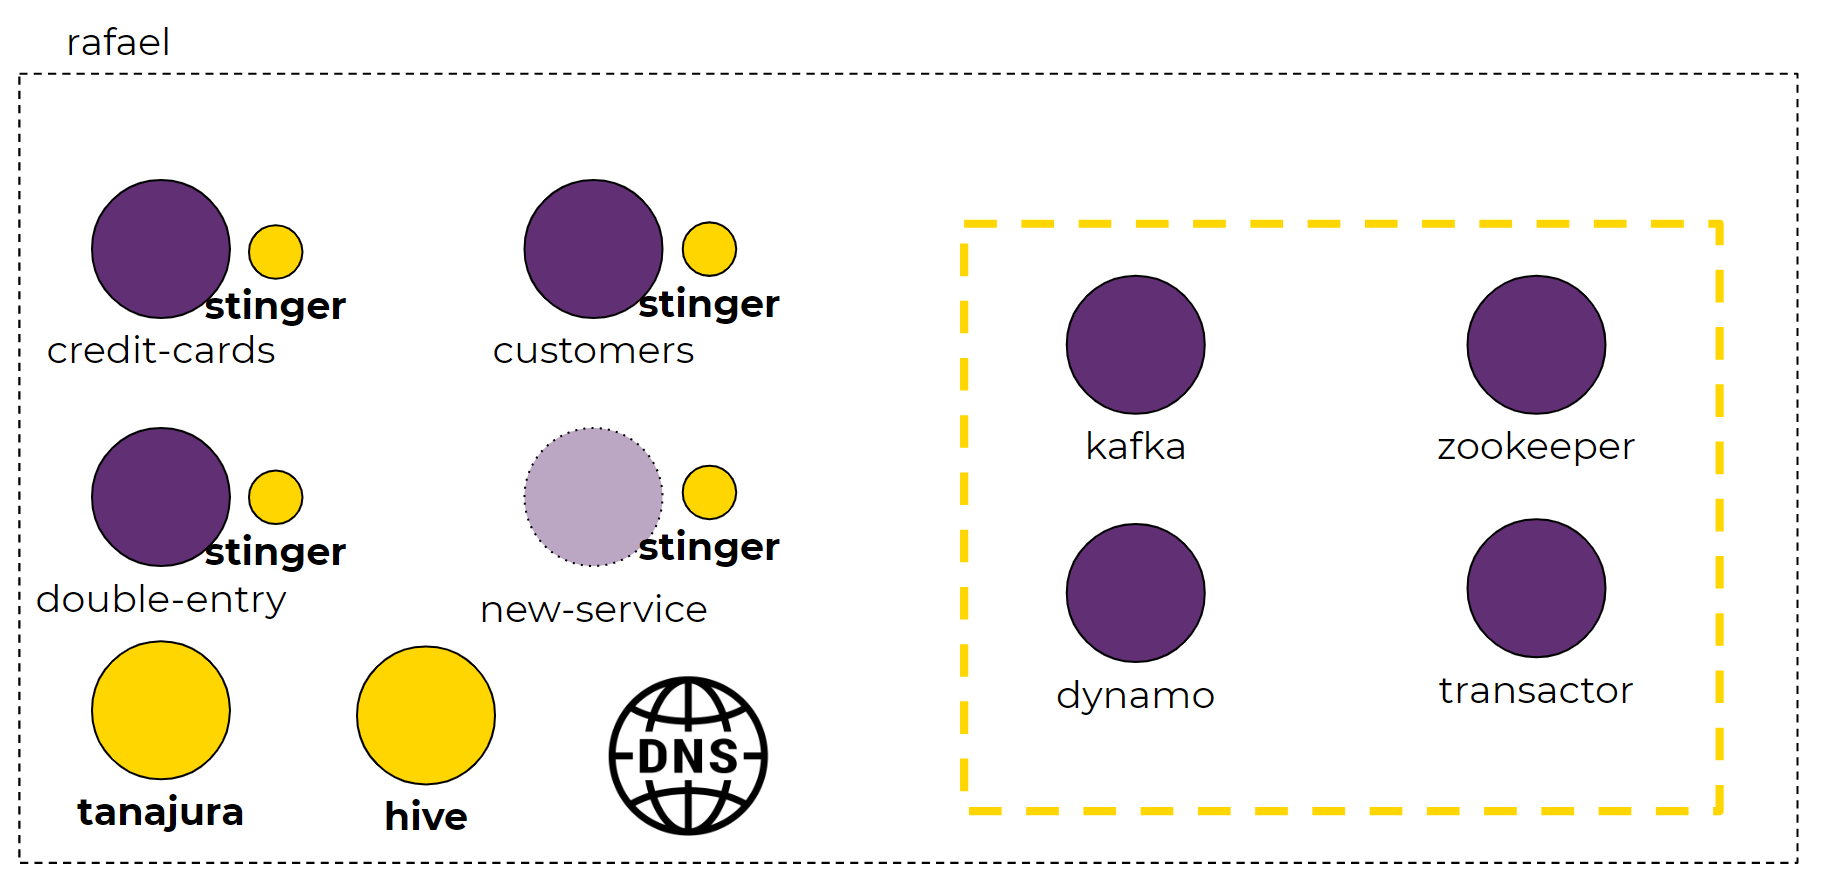
\includegraphics[scale=0.30]{pictures/devspace1.png}
			\end{center}
			\legend{Fonte: os autores}
			% \caption{Fonte: própria}
		\end{figure}
    
    	\begin{figure}[htbp]
			\caption{\label{fig_create_devspace}Fluxo de Criação de Devspaces}
			\begin{center}
			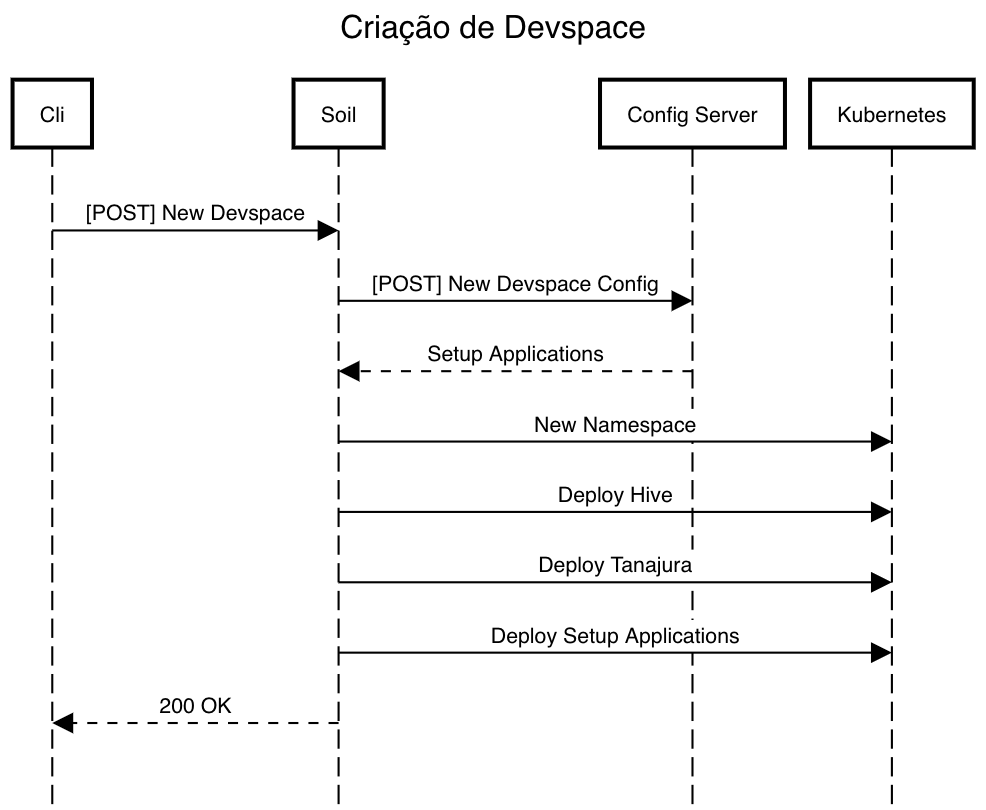
\includegraphics[scale=0.40]{pictures/create-devspace.png}
			\end{center}
			\legend{Fonte: os autores}
			% \caption{Fonte: própria}
		\end{figure}

	\section{FileSync}

	Um dos grandes desafios do projeto foi a construção de um sistema para sincronização de arquivos em uma arquitetura distribuída de microsserviços.
	
	O caso de uso principal para esta funcionalidade é permitir que o engenheiro da Nubank pudesse iterar de maneira mais rápida no desenvolvimento de um novo microsserviço ou em modificações de algum existente.
	
	Do ponto de vista da empresa, esta era um dos requisitos mais desejados e que mais agregaria valor ao produto final, dado que é uma ferramenta extremamente poderosa para o engenheiro, garantindo-lhe mais produtividade e liberdade enquanto estivesse desenvolvendo.
	
	Este sistema de sincronização de arquivos precisava atender algumas premissas:
	- Deve se integrar facilmente ao workflow do engenheiro, para haver um incentivo à sua adoção.
	- Segurança: Os arquivos trafegados não devem ser, de maneira alguma, expostos para a internet ou suscetíveis a ataques como Man in the middle, dado que o conteúdo trafegado é extremamente sensível (códigos fonte dos produtos da empresa)
	- Velocidade: Quanto mais rápido for o processo de sincronização, mais dinâmico será o processo, permitindo iterações mais rápidas e, consequentemente, maior produtividade.

	Para entender o problema que o sistema de Filesync se propõe a resolver, é preciso entender o cenário:
	
	Os serviços em que o engenheiro está trabalhando não estão sendo compilados e executados na mesma máquina em que está o código fonte. Na verdade eles estão sendo executados em um contêiner Docker, gerenciado por um \textit{cluster} Kubernetes, operando em uma infraestrutura de \textit{hardware} fornecida pela AWS EC2. Para que mudanças no código fonte fossem de fato percebidas pelo desenvolvedor, este precisaria compilar uma nova imagem Docker com o código fonte atualizado, publica-lá em um repositório de contêineres e realizar a implantação desta nova imagem no \textit{cluster} remoto. Este processo, em um contexto de desenvolvimento, é extremamente ineficiente, o que tornaria a ferramenta pouco dinâmica e não atrativa para o engenheiro.

	Para evitar a geração de uma nova imagem Docker a cada iteração no código fonte, foi desenvolvida uma imagem genérica capaz de compilar e executar qualquer serviço da Nubank em modo de desenvolvimento. Esta imagem foi apelidada de Chamber e uma de suas características é a sua extensibilidade, permitindo que em melhorias futuras sejam desenvolvidas versões para outras linguagens e plataformas (Como por exemplo \textit{NodeJS}, \textit{Ruby}, \textit{Scala}, \textit{etc.}). Para implantação no Nubank, foi desenvolvida a imagem Chamber-lein, capaz de executar programas escritos em \textit{Clojure}, principal linguagem utilizada nos microsserviços do Nubank.
	
	Além disto, esta imagem tem um componente de software capaz de atualizar o código do serviço que está sendo executado dentro do contêiner através do Git.
	
% 	\section{Arquitetura da solução}
% 		\begin{figure}[htb]
% 			\caption{\label{fig_arquitetura1}Arquitetura da solução}
% 			\begin{center}
% 			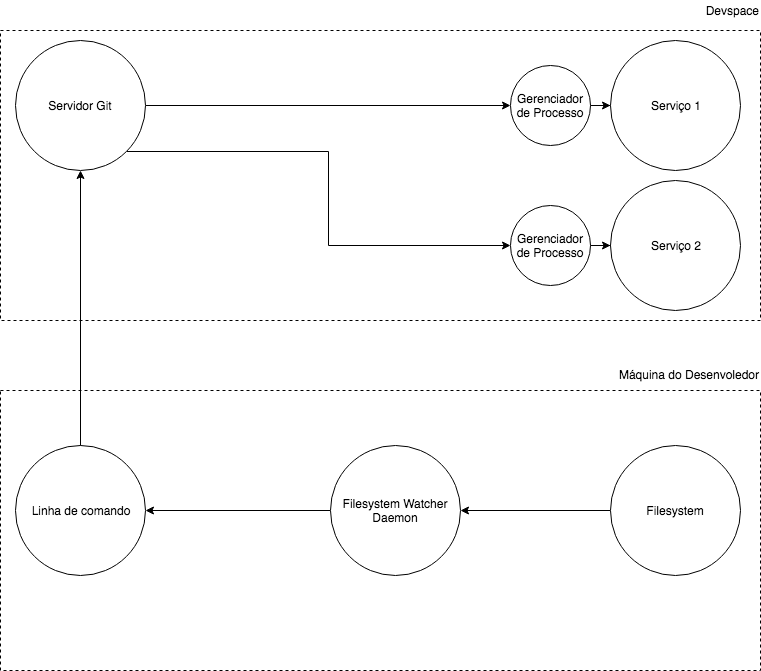
\includegraphics[scale=0.50]{pictures/arquitetura-da-solucao.png}
% 			\end{center}
% 			\legend{Fonte: os autores}
% 		\end{figure}
	
	\subsection{Servidor web para Git (Tanajura)}
	Um dos componentes do sistema de sincronização de arquivos é um servidor web apelidado de \textit{Tanajura}. O serviço tem como principal responsabilidade ser um \textit{hub} de repositórios Git.
	
	Nestes repositórios está o código fonte dos serviços em que o desenvolvedor está trabalhando no momento e o Git é utilizado como mecanismo de sincronização entre o sistema de arquivos local da máquina do desenvolvedor e o sistema de arquivos do contêiner em que está sendo executado a aplicação, em um \textit{cluster} Kubernetes remoto.
	
	O serviço conta com \textit{endpoints} para gerenciamento de repositórios (operações de criação, remoção e consulta) através de uma interface REST, bem como um \textit{endpoint} que implementa os protocolos do Git para transferência e dados através de HTTP. Assim é possível para qualquer cliente Git a realização das operações básicas como \textit{push}, \textit{pull} e \textit{fetch}.
	
	Os repositórios Git neste serviço têm como característica a efemeridade, ou seja, eles não precisam ser de mecanismos robustos de persistência e só existem para fins de sincronização entre dois sistemas de arquivos, podendo ser sobrescritos e apagados a qualquer momento sem perda de dados importantes.
	
	A escolha do Git para este sistema de sincronização pode ser justificado por algumas de suas características que atendiam os requisitos definidos:
	
	- O binário do Git já está presente na máquina do desenvolvedor do Nubank, pois todos trabalham com Git em seu dia-a-dia.
	
	- É um método eficiente para troca de dados, pois os \textit{commits} são criados a partir das modificações feitas em arquivos, ou seja, apenas as diferenças são transmitidas pela rede.
	
	- A troca de dados pode ser criptografada com SSL.

	Ao receber um \textit{push} em algum repositório Git, o \textit{Tanajura} identifica qual o serviço associado ao repositório e faz uma requisição HTTP para o \textit{Soil} a fim de obter a URL do Gerenciador de Processo (\textit{Stinger}) deste serviço.
	
	Uma vez obtida esta URL, o serviço \textit{Tanajura} faz uma requisição para o \textit{Stinger} avisando-o de que há uma nova versão do código disponível para ser sincronizada.
	
	Este, por sua vez, realiza um \textit{pull} no repositório remoto para obtenção do código atualizado e, após o recebimento dos arquivos, executa os \textit{scripts} necessários para recompilação e execução do código.
	
	Esta parte do processo pode ser representada pelo seguinte diagrama de sequência:
		\begin{figure}[htb]
			\caption{\label{fig_arquitetura2}Fluxo do Tanajura}
			\begin{center}
			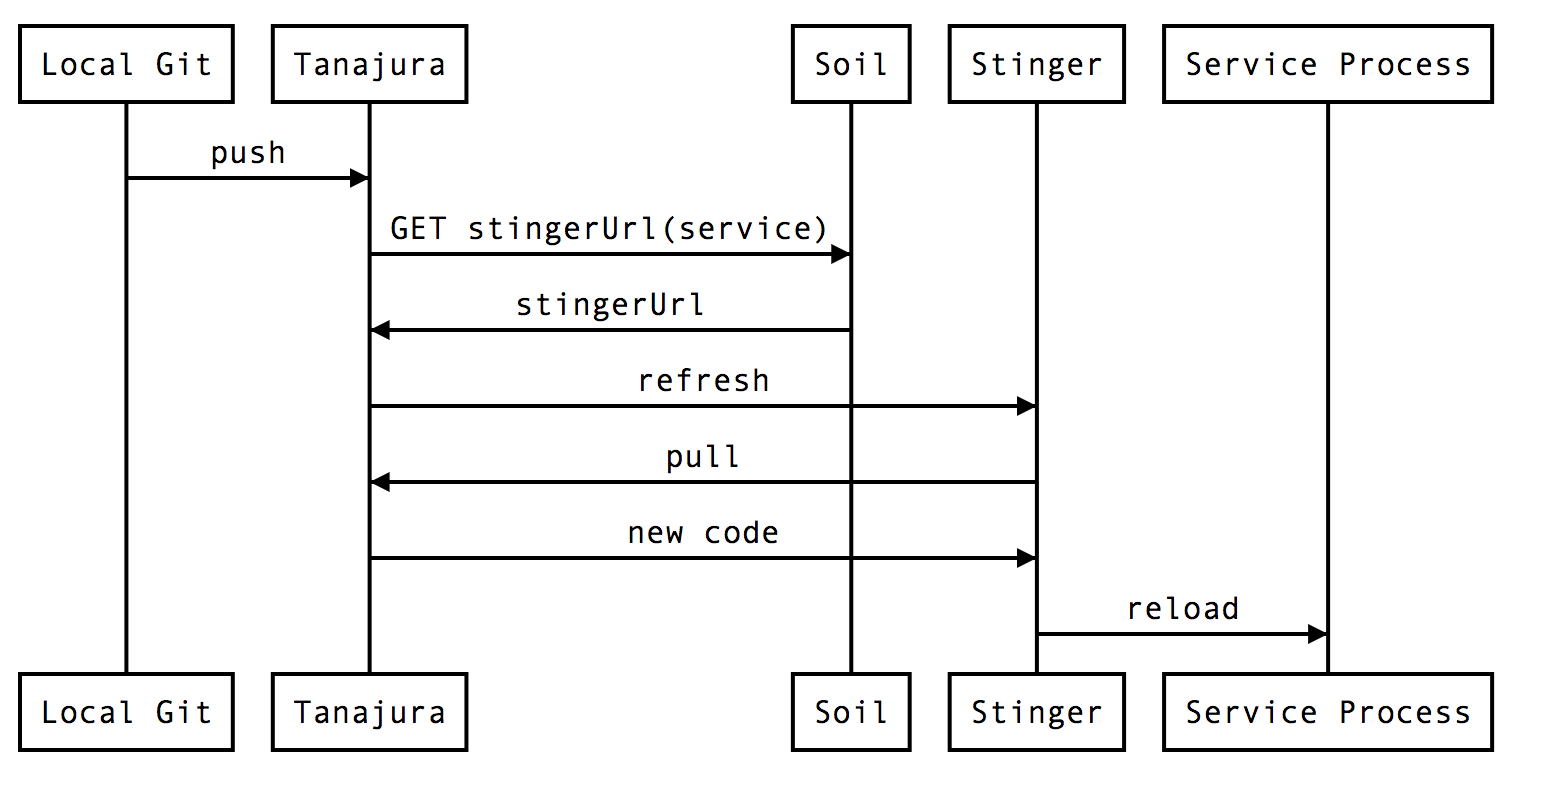
\includegraphics[scale=0.29]{pictures/tanajura-flow.png}
			\end{center}
			\legend{Fonte: os autores}
			% \caption{Fonte: própria}
		\end{figure}

	Em termos práticos, o processo ocorre da seguinte maneira:
	
	Quando o desenvolvedor deseja implantar em seu devspace um serviço com capacidades de sincronização, ele digita o seguinte o comando:

	\begin{verbatim}
	fmc service:deploy:local my-service -f ./config.json /path/to/service
	\end{verbatim}

	Este comando irá realizar a implantação de um serviço chamado \textit{"my-service"}, utilizando o arquivo de configuração \textit{"./config.json"} a partir da pasta local \textit{"/path/to/service"}

	\subsection{Gerenciador de Processos (Stinger)}	
	
	Para que fosse possível o método de sincronização de arquivos utilizando Git foi necessário o desenvolvimento de uma aplicação que, através de uma interface HTTP exposta para o \textit{cluster}, pudesse fazer \textit{pull} em um repositório Git remoto para obtenção do código fonte atualizado e, após o recebimento dos arquivos, fosse possível executar um comando arbitrário para que o processo do serviço pudesse ser recarregado.
	
	Esta aplicação foi apelidada de Stinger e é o binário executado primariamente pela imagem Docker onde os serviços são executados (esta imagem será descrita em detalhes mais adiante). Os endpoints HTTP disponíveis neste serviço são:

    \textbf{POST /reset}
	\newline
	Ao receber uma requisição neste endpoint, o Stinger termina o processo do serviço em execução através de seu identificador de processo (\textit{process ID}) e executa o \textit{script} de \textit{cleanup}. Após a garantia de que o processo do serviço foi terminado com êxito, é executado o \textit{script} de \textit{start}, que garante sua reinicialização.
	
	\textbf{POST /pull}
	\newline
	Ao receber uma requisição neste endpoint, o Stinger executa o comando git pull origin master para obter a versão mais recente do código no repositório remoto. É possível, através de parâmetros no corpo da requisição, fazer com que o processo do serviço seja reinicializado logo após o recebimento do código atualizado.

	Quando o Stinger é iniciado, ele verifica a existência do repositório Git local e, caso não o encontre, executa o comando \textit{git clone [url do repositório] [pasta local]} para obter a versão inicial do código. Logo após o recebimento dos arquivos, é feito o processo de inicialização do serviço.

	É possível configurar diversos parâmetros de funcionamento do \textit{Stinger} através de variáveis de ambiente. Os mais relevantes são:
	
	\textbf{APP\_PATH}
	\newline
	É a o caminho para o diretório local onde o Stinger irá clonar o código do repositório remoto.
	
	\textit{exemplo: /app}

	\textbf{STINGER\_SCRIPTS}
	\newline
	Caminho para o diretório local onde o Stinger irá executar os scripts para gerenciar os ciclos de vida do serviço. Dentro desta pasta, devem estar presentes os scripts de start e cleanup.
	
	\textit{exemplo: /scripts}
	
	\textbf{GIT\_URL}
	\newline
	É a URL de onde o \textit{Stinger} fará o \textit{git clone} inicial dos arquivos.
	
	\textit{exemplo: \url{https://tanajura.joe.formicarium.nubank.com.br/service-name}}
	
	\textbf{START\_AFTER\_PULL}
	\newline
	Caso esta variável esteja setada, o \textit{Stinger} irá reinicializar o processo sempre após o recebimento de novo código através do \textit{pull}. Esta configuração existe porque em certas linguagens de programação (como a utilizada pela Nubank) não é necessário recompilar e nem executar nenhum comando para que o novo código obtido seja aplicado no processo em execução.
    
	De maneira geral, o \textit{Stinger} é um gerenciador de processos integrado com o Git e que expõe suas funcionalidades através de um servidor HTTP.

\section{Frontend}  
    \subsection{Organização do código}
Para oferecer uma interface amigável aos usuários, foram construídas duas aplicações: uma Interface de linha de comando e uma Aplicação \textit{Desktop}. Ambas têm funcionalidades semelhantes, porém a segunda oferece elementos de interface gráfica essenciais para a construção do módulo de \textit{Distributed Debugger} do sistema.

Como as duas aplicações compartilham diversos módulos, todo o código comum foi extraído para uma biblioteca (chamada \textit{common}) e seu código fica disponível para ambas as aplicações através de um sistema de dependências oferecido pelo NPM.

Foi tomado o cuidado de não se criar acoplamentos dos módulos desta biblioteca com casos de uso específicos de cada aplicação, tornando o código mais reaproveitável e desacoplado, com responsabilidades bem definidas.

O código dos três módulos vive em mesmo repositório Git, dividido apenas por pastas. Esta prática é comum para o gerenciamento de múltiplos módulos que compõe um sistema maior e  repositórios com esta característica são denominados \textit{monorepos}.

Este tipo de organização é vantajosa pois preserva os benefícios de desacoplamento das diferentes partes do sistema, porém eliminando, através do uso de ferramentas específicas, as complexidades de se gerenciar as dependências entre os diversos módulos, tanto no estágio de desenvolvimento quanto nos estágios de compilação e publicação.

Para gerenciar as dependências do \textit{monorepo}, foi utilizado a ferramenta \textit{yarn workspaces}, que otimiza o uso de memória em disco do código fonte e o tempo de instalação inicial para novos desenvolvedores através do compartilhamento das dependências comuns entre os vários módulos. Ela também é responsável por criar \textit{links} simbólicos (\textit{symlinks}) entre os módulos quando em estágio de desenvolvimento. Os \textit{symlinks} permitem iterações mais rápidas de desenvolvimento, pois uma mudança no código de uma dependência irá refletir automaticamente nos módulos dependentes, sem a necessidade de se incrementar versões e recompilar partes do programa.

Todos os módulos do projeto utilizam \textit{Semantic Versioning} como padrão versionamento. O incremento é feito automaticamente através de uma ferramenta que analisa as mensagens presentes nos commits do Git para determinar, através de \textit{tokens} pré-definidos, qual será o incremento de versão: \textit{Major}, \textit{minor}, \textit{patch}.

Além do incremento automático em cada módulo, foi utilizada a ferramenta \textit{Lerna} para determinar quais módulos e dependências devem ter suas versões atualizadas, através também da análise de quais arquivos foram modificados nos commits desde a última atualização.

Todo este ferramental tornou a experiência de desenvolvimento deste projeto muito mais eficiente e facilitará também sua manutenção.

    \subsection{Interface de linha de comando}
    Para a construção deste software, foi utilizado a linguagem Typescript, com a plataforma NodeJS. A framework para desenvolvimento foi a ocli, mantida pela Salesforce.
    Este software é distribuído através do NPM (\textit{Node Package Manager)}. Por ser uma ferramenta já presente nos computadores dos engenheiros do Nubank, a instalação da linha de comando se torna simples e rápida, basta executar o comando
    \begin{verbatim}
	npm install -g @formicarium/cli
	\end{verbatim}
	
	Com isso, o binário \textit{fmc} já fica disponível para ser executado através do terminal.
	
	Para atualizar a versão do software após a publicação de alguma modificação, basta o comando
	\begin{verbatim}
	npm update -g @formicarium/cli
	\end{verbatim}
	
	Este mecanismo de fácil distribuição e atualização foi escolhido para facilitar ainda mais a adesão dos engenheiros ao uso do ecossistema Formicarium.

A interface de linha de comando apresenta suas funcionalidades divididas em subprogramas, cada um referente a um conjunto de casos de uso agrupados logicamente. Utilizando o comando \textit{help}, o engenheiro tem acesso à documentação da ferramenta, podendo listar os subprogramas e comandos disponíveis dentro de cada nível hierárquico de funcionalidades e entender o que fazem através de descrições e exemplos de uso.

Por exemplo, ao requisitar ajuda no contexto geral da linha de comando:

\begin{verbatim}
A CLI to operate on Formicarium
VERSION
    @formicarium/cli/1.3.2 darwin-x64 node-v11.1.0
USAGE
    $ fmc [COMMAND]
COMMANDS
    devspace  Creates a Devspace
    git       Configures local fmcgit and hive
    help      display help for fmc
    repl      Connects to remote repl. If no service is provided, connects on Hive's Repl
    service   Deletes a service in the current Devspace
    setup     Configures Formicarium CLI to one cluster
\end{verbatim}

Ao requisitar ajuda para um contexto específico (no caso, o contexto \textit{devspace}):
\begin{verbatim}
Creates a Devspace

USAGE
  $ fmc devspace:COMMAND

COMMANDS
  devspace:create    Creates a Devspace
  devspace:delete    Deletes a Devspace
  devspace:info      Get information for the current devspace
  devspace:list      List availables Devspaces
  devspace:services  Lists the services in your devspace
  devspace:use       Configures to use one Devspace context
\end{verbatim}


Ao requisitar ajuda para um comando específico (no caso, o comando \textit{devspace:create}):
\begin{verbatim}
Creates a Devspace

USAGE
  $ fmc devspace:create ID

OPTIONS
  -h, --help  show CLI help
  --test

EXAMPLE
  $ fmc devspace:create paps
\end{verbatim}


A facilidade proporcionada ao engenheiro do Nubank para entender o uso da ferramenta através desta documentação interativa fez parte da estratégia do grupo para disseminação e adesão da ferramenta por toda a empresa de maneira escalável.

Lista de comandos disponíveis e uma breve descrição do que fazem

devspace
  devspace:create    Creates a Devspace
  devspace:delete    Deletes a Devspace
  devspace:info      Get information for the current devspace
  devspace:list      List availables Devspaces
  devspace:services  Lists the services in your devspace
  devspace:use       Configures to use one Devspace context
  

sync
  sync:push   Configures local fmcgit and hive
  sync:setup  Deploys service

repl

service
  service:delete   Deletes a service in the current Devspace
  service:deploy   Deploys service
  service:logs     A service logs in the current Devspace
  service:restart  Restart a service deployed in dev mode
  service:status   Restart a service deployed in dev mode
  

setup




    \subsection{Aplicação \textit{Desktop}}

Como parte do ferramental do ambiente Formicarium, foi desenvolvida uma aplicação Desktop multiplataforma (Windows, Linux, OS X) com o intuito de melhorar a experiência dos usuários nas funções mais comuns e também para atender requisitos do sistema que exigiam interfaces gráficas mais interativas e avançadas. A aplicação foi desenvolvida utilizando tecnologias web (HTML5, CSS3 e Javascript), o que tornou possível sua execução em diferentes plataformas utilizadas pelos engenheiros do Nubank. Como era necessário o uso de \textit{APIs} nativas do sistema (como acesso ao sistema de arquivos e execução de outros programas a partir da interface gráfica) que não seriam possível no browser, foi utilizada a \textit{framework} Electron para empacotar a aplicação em um binário capaz de ter acesso às \textit{system calls} necessárias. Electron é a framework por trás de diversos projetos populares como Slack, WhatsApp Desktop, Visual Studio Code, Atom, Spotify entre outros. Além disso, conta com uma enorme comunidade, melhorando ainda as características de manutenibilidade de software da solução.

Para a sua distribuição dentro do Nubank, o software compilado foi disponibilizado em um \textit{bucket} da \textit{AWS S3} acessível apenas para funcionários credenciados \textit{download} e execução para começar a utilizá-lo.

A aplicação ainda não conta com sistemas automatizados de atualização, sendo necessária a obtenção manual de uma nova versão sempre que o engenheiro veja a necessidade de atualização. Este mecanismo de atualização poderá ser aprimorado em melhoria futuras.

\subsection{Gerenciamento de Devspaces}
Esta área tem como objetivo mostrar ao engenheiro os Devspaces disponíveis para serem utilizados. Normalmente o Devspace pessoal do engenheiro estará selecionado, porém é possível por exemplo alternar entre este e o Devspace do \textit{squad} ou ainda o de algum colega caso queiram compartilhar alguma configuração para reproduzir ambientes de testes e desenvolvimento.

\begin{figure}[htb]
	\caption{\label{fig_frontend_devspaces}Tela Lista de Devspaces}
	\begin{center}
	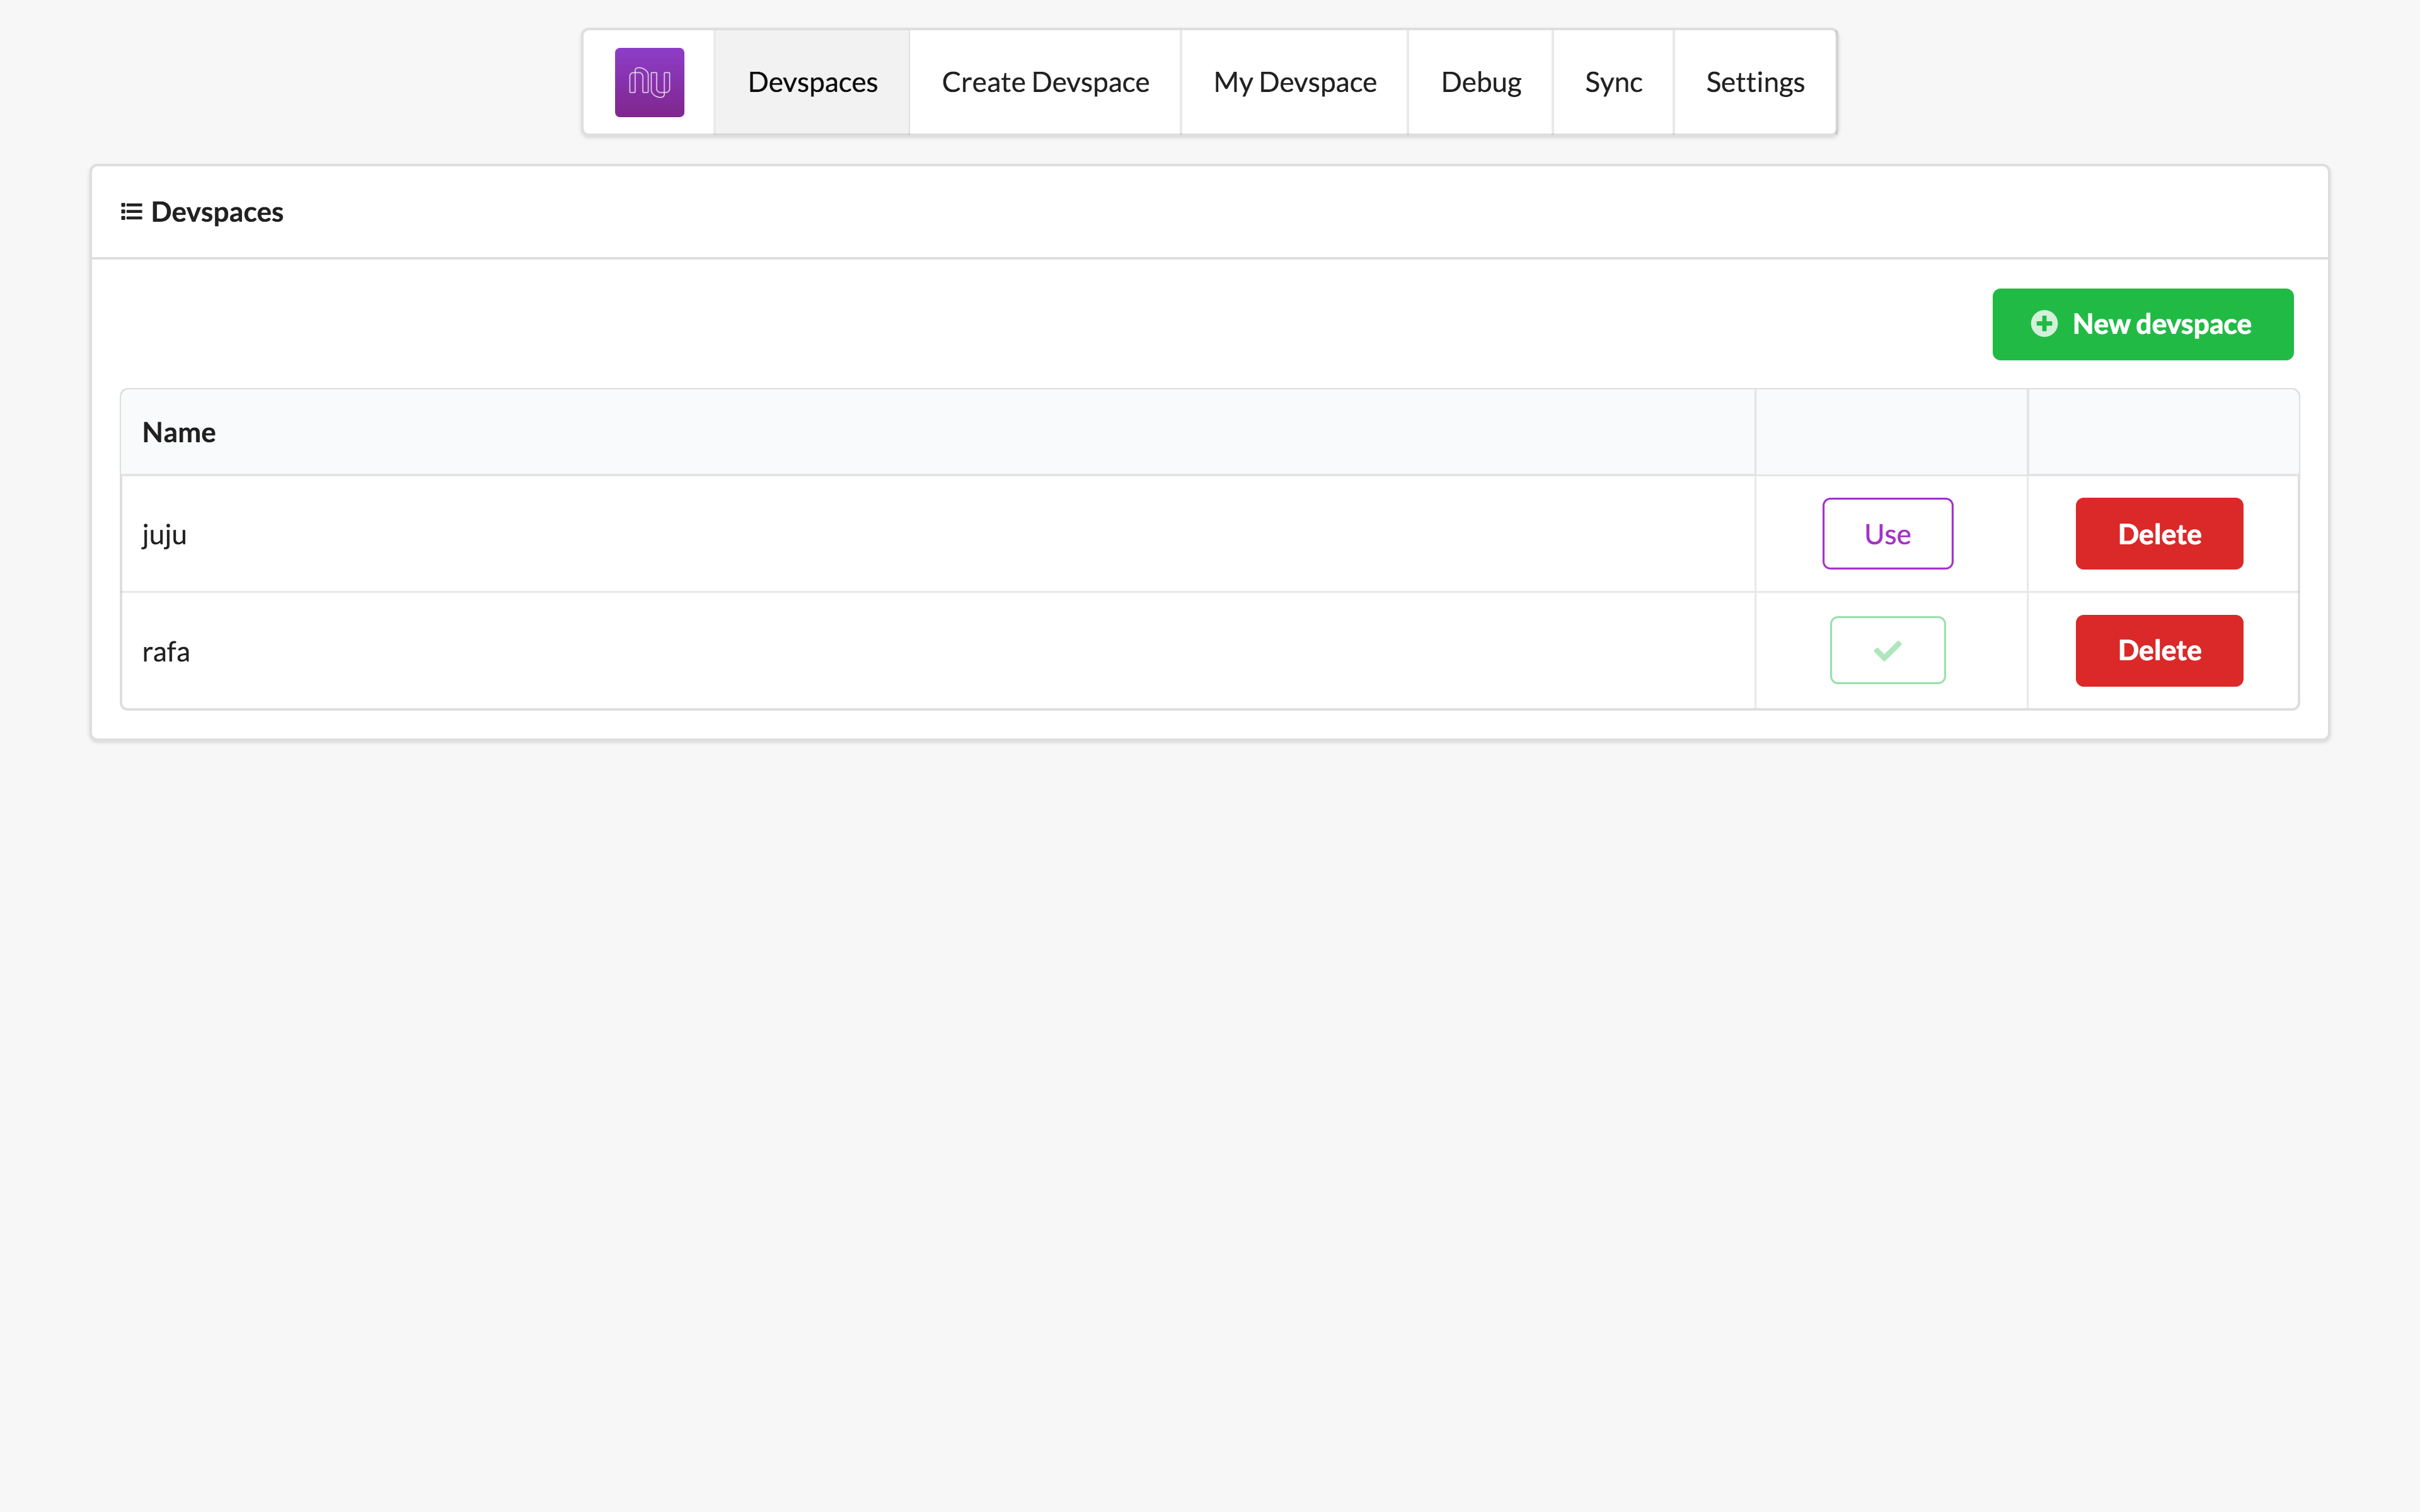
\includegraphics[width=\textwidth,keepaspectratio]{pictures/frontend/frontend-devspaces.png}
	\end{center}
	\legend{Fonte: Elaborado pelos autores}
\end{figure}



\subsection{Devspace}
Esta área tem como objetivo mostrar informações e proporcionar interações com o Devspace específico selecionado pelo engenheiro.

\subsubsection{Infraestrutura}
Nesta área o engenheiro pode conferir o status dos serviços básicos de infraestrutura do Devspace, como o Hive (para \textit{Distributed Tracing}) e o Tanajura (para sincronização de arquivos). Também é possível extrair os logs destes serviços em tempo real.

\begin{figure}[htb]
	\caption{\label{fig_frontend_devspace_info}Tela Informações do Devspace}
	\begin{center}
	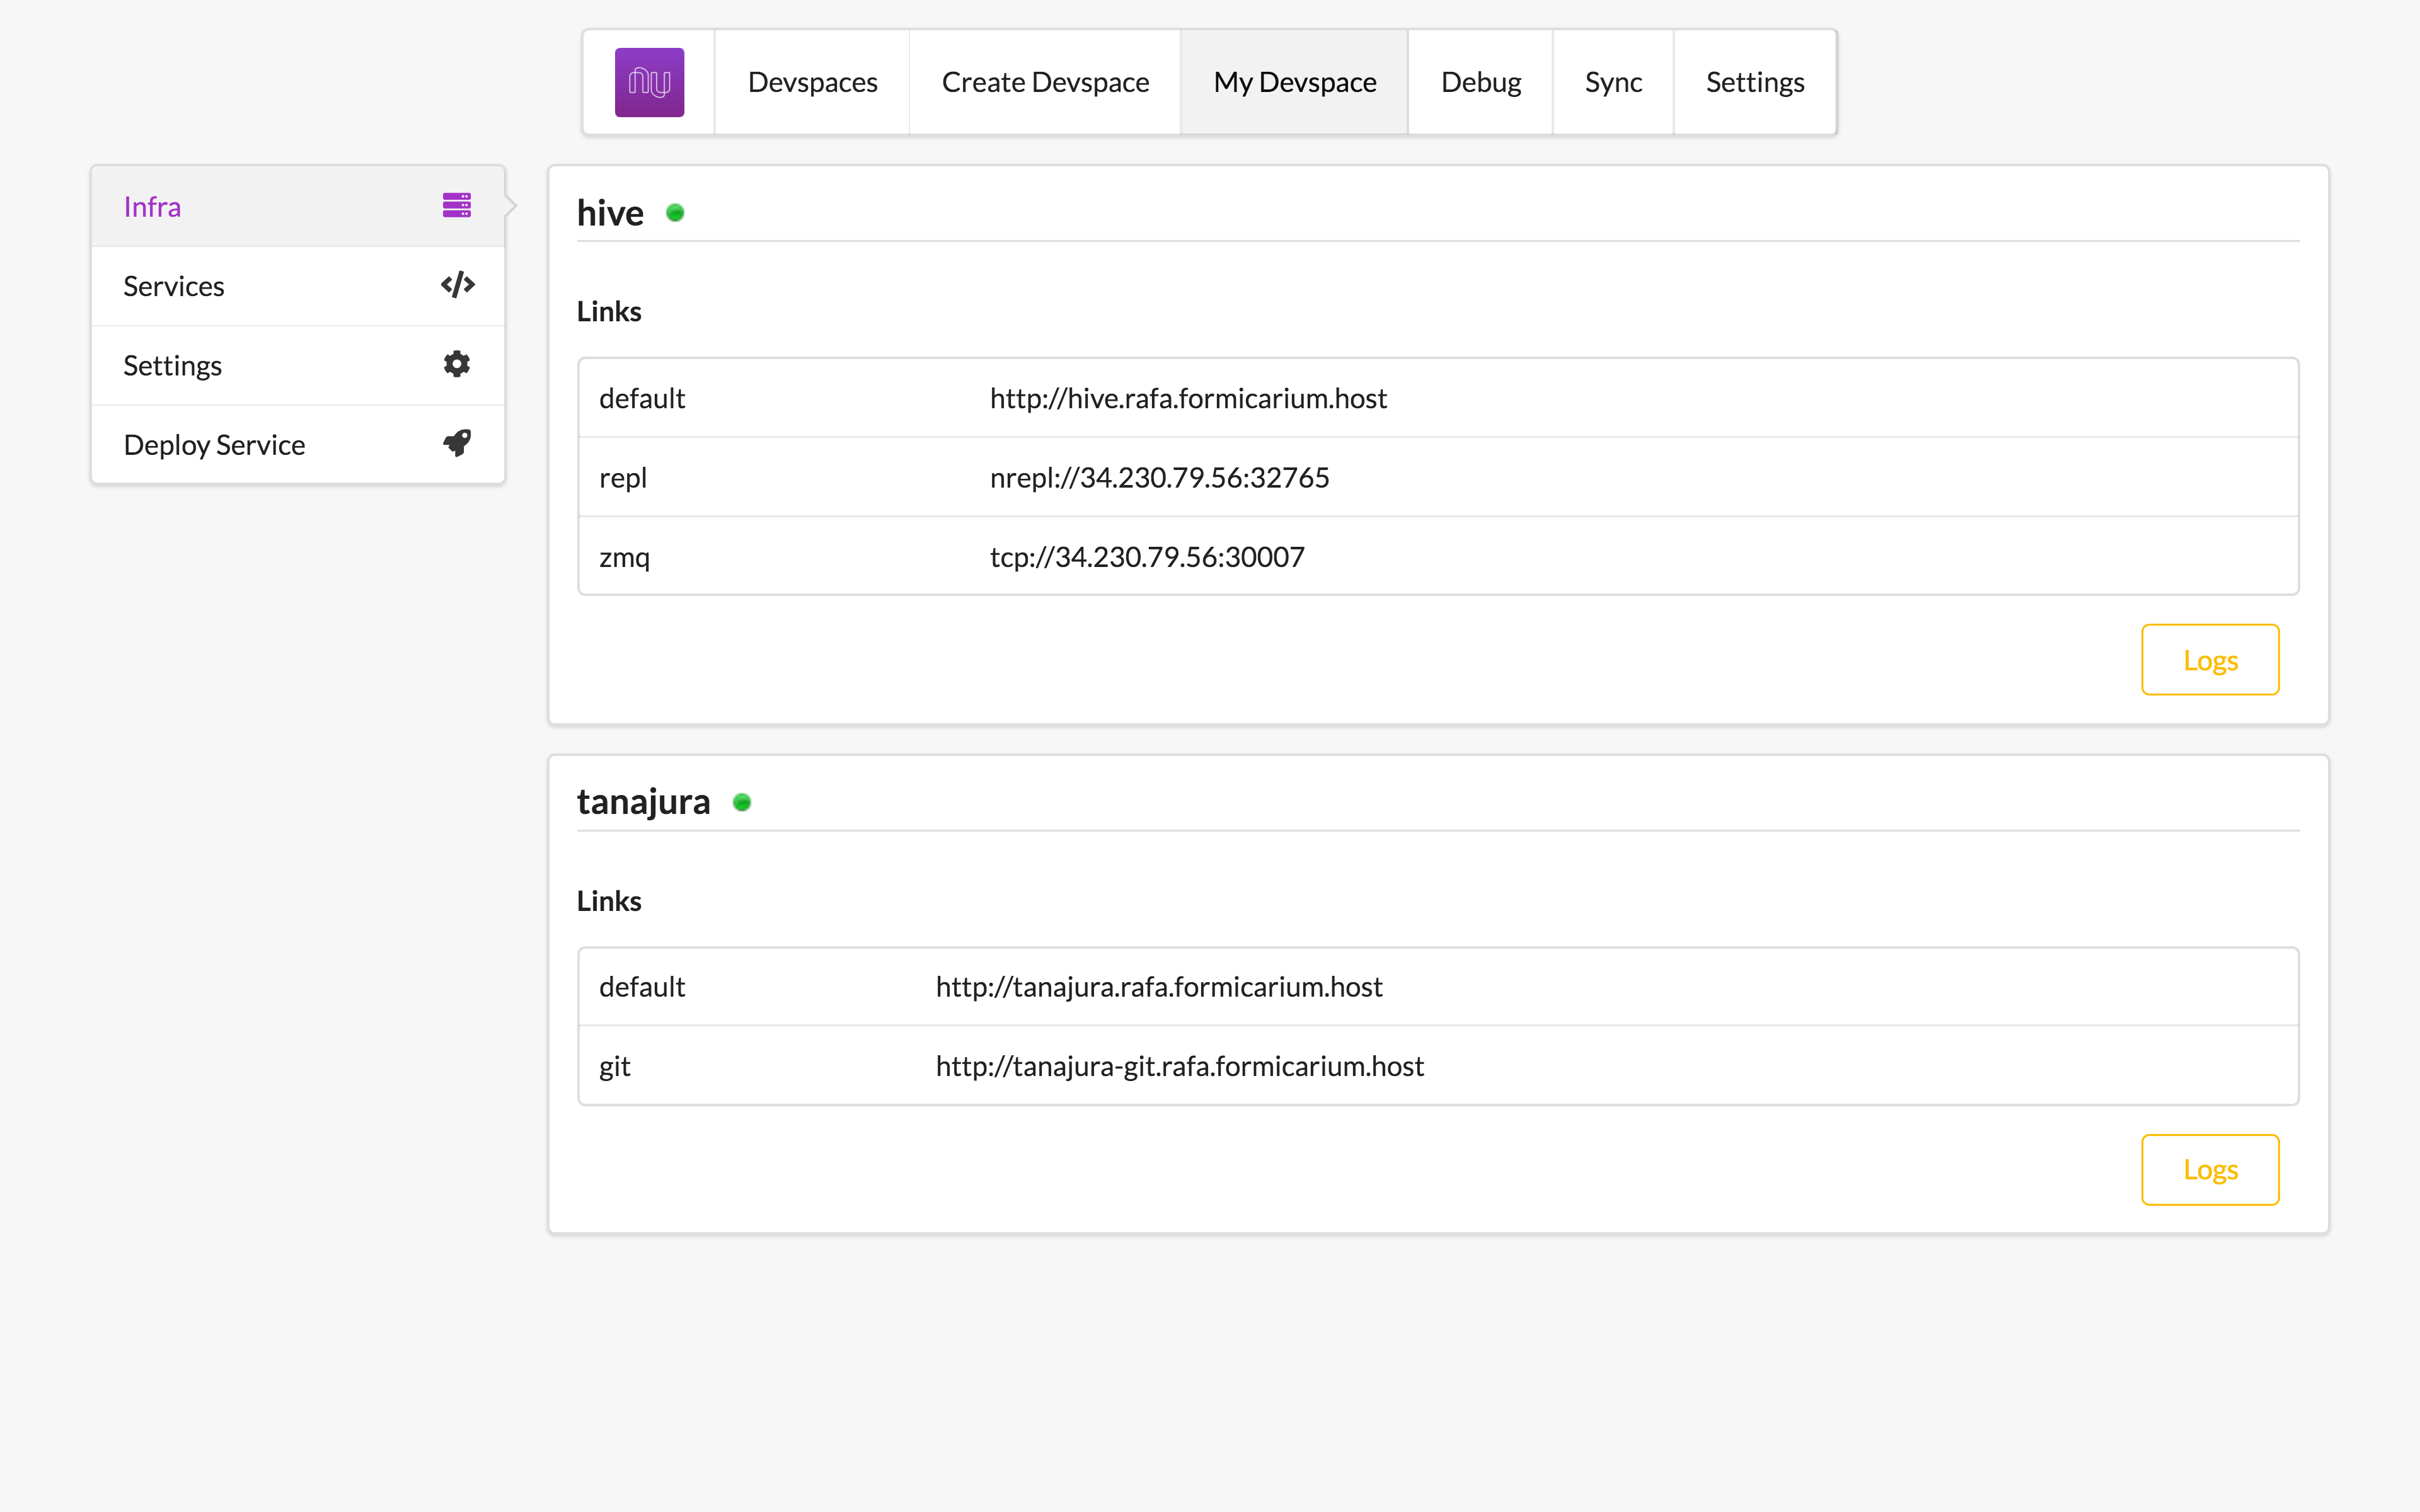
\includegraphics[width=\textwidth,keepaspectratio]{pictures/frontend/frontend-devspace-info.png}
	\end{center}
	\legend{Fonte: Elaborado pelos autores}
\end{figure}

\subsubsection{Serviços}

Nesta área o engenheiro pode conferir o status dos serviços implantados no Devspace atual e também interagir com cada um deles de forma independente. É possível a obtenção em tempo real dos \textit{logs} (tudo que for direcionado ao \textit{stdout} e \textit{stderr} do processo), a reinicialização do processo e também a sua remoção do Devspace através de botões. A lista também apresenta as interfaces de cada processo expostas para a \textit{internet} para permitir outros tipos de interação, como por exemplo a interface de um possível servidor HTTP do serviço e a interface HTTP do Stinger, que é um gerenciador de processos oferecido pelo Formicarium e que está presente nos serviços implantados no Devspace.

\begin{figure}[htb]
	\caption{\label{fig_frontend_devspace_services}Tela Serviços do Devspace}
	\begin{center}
	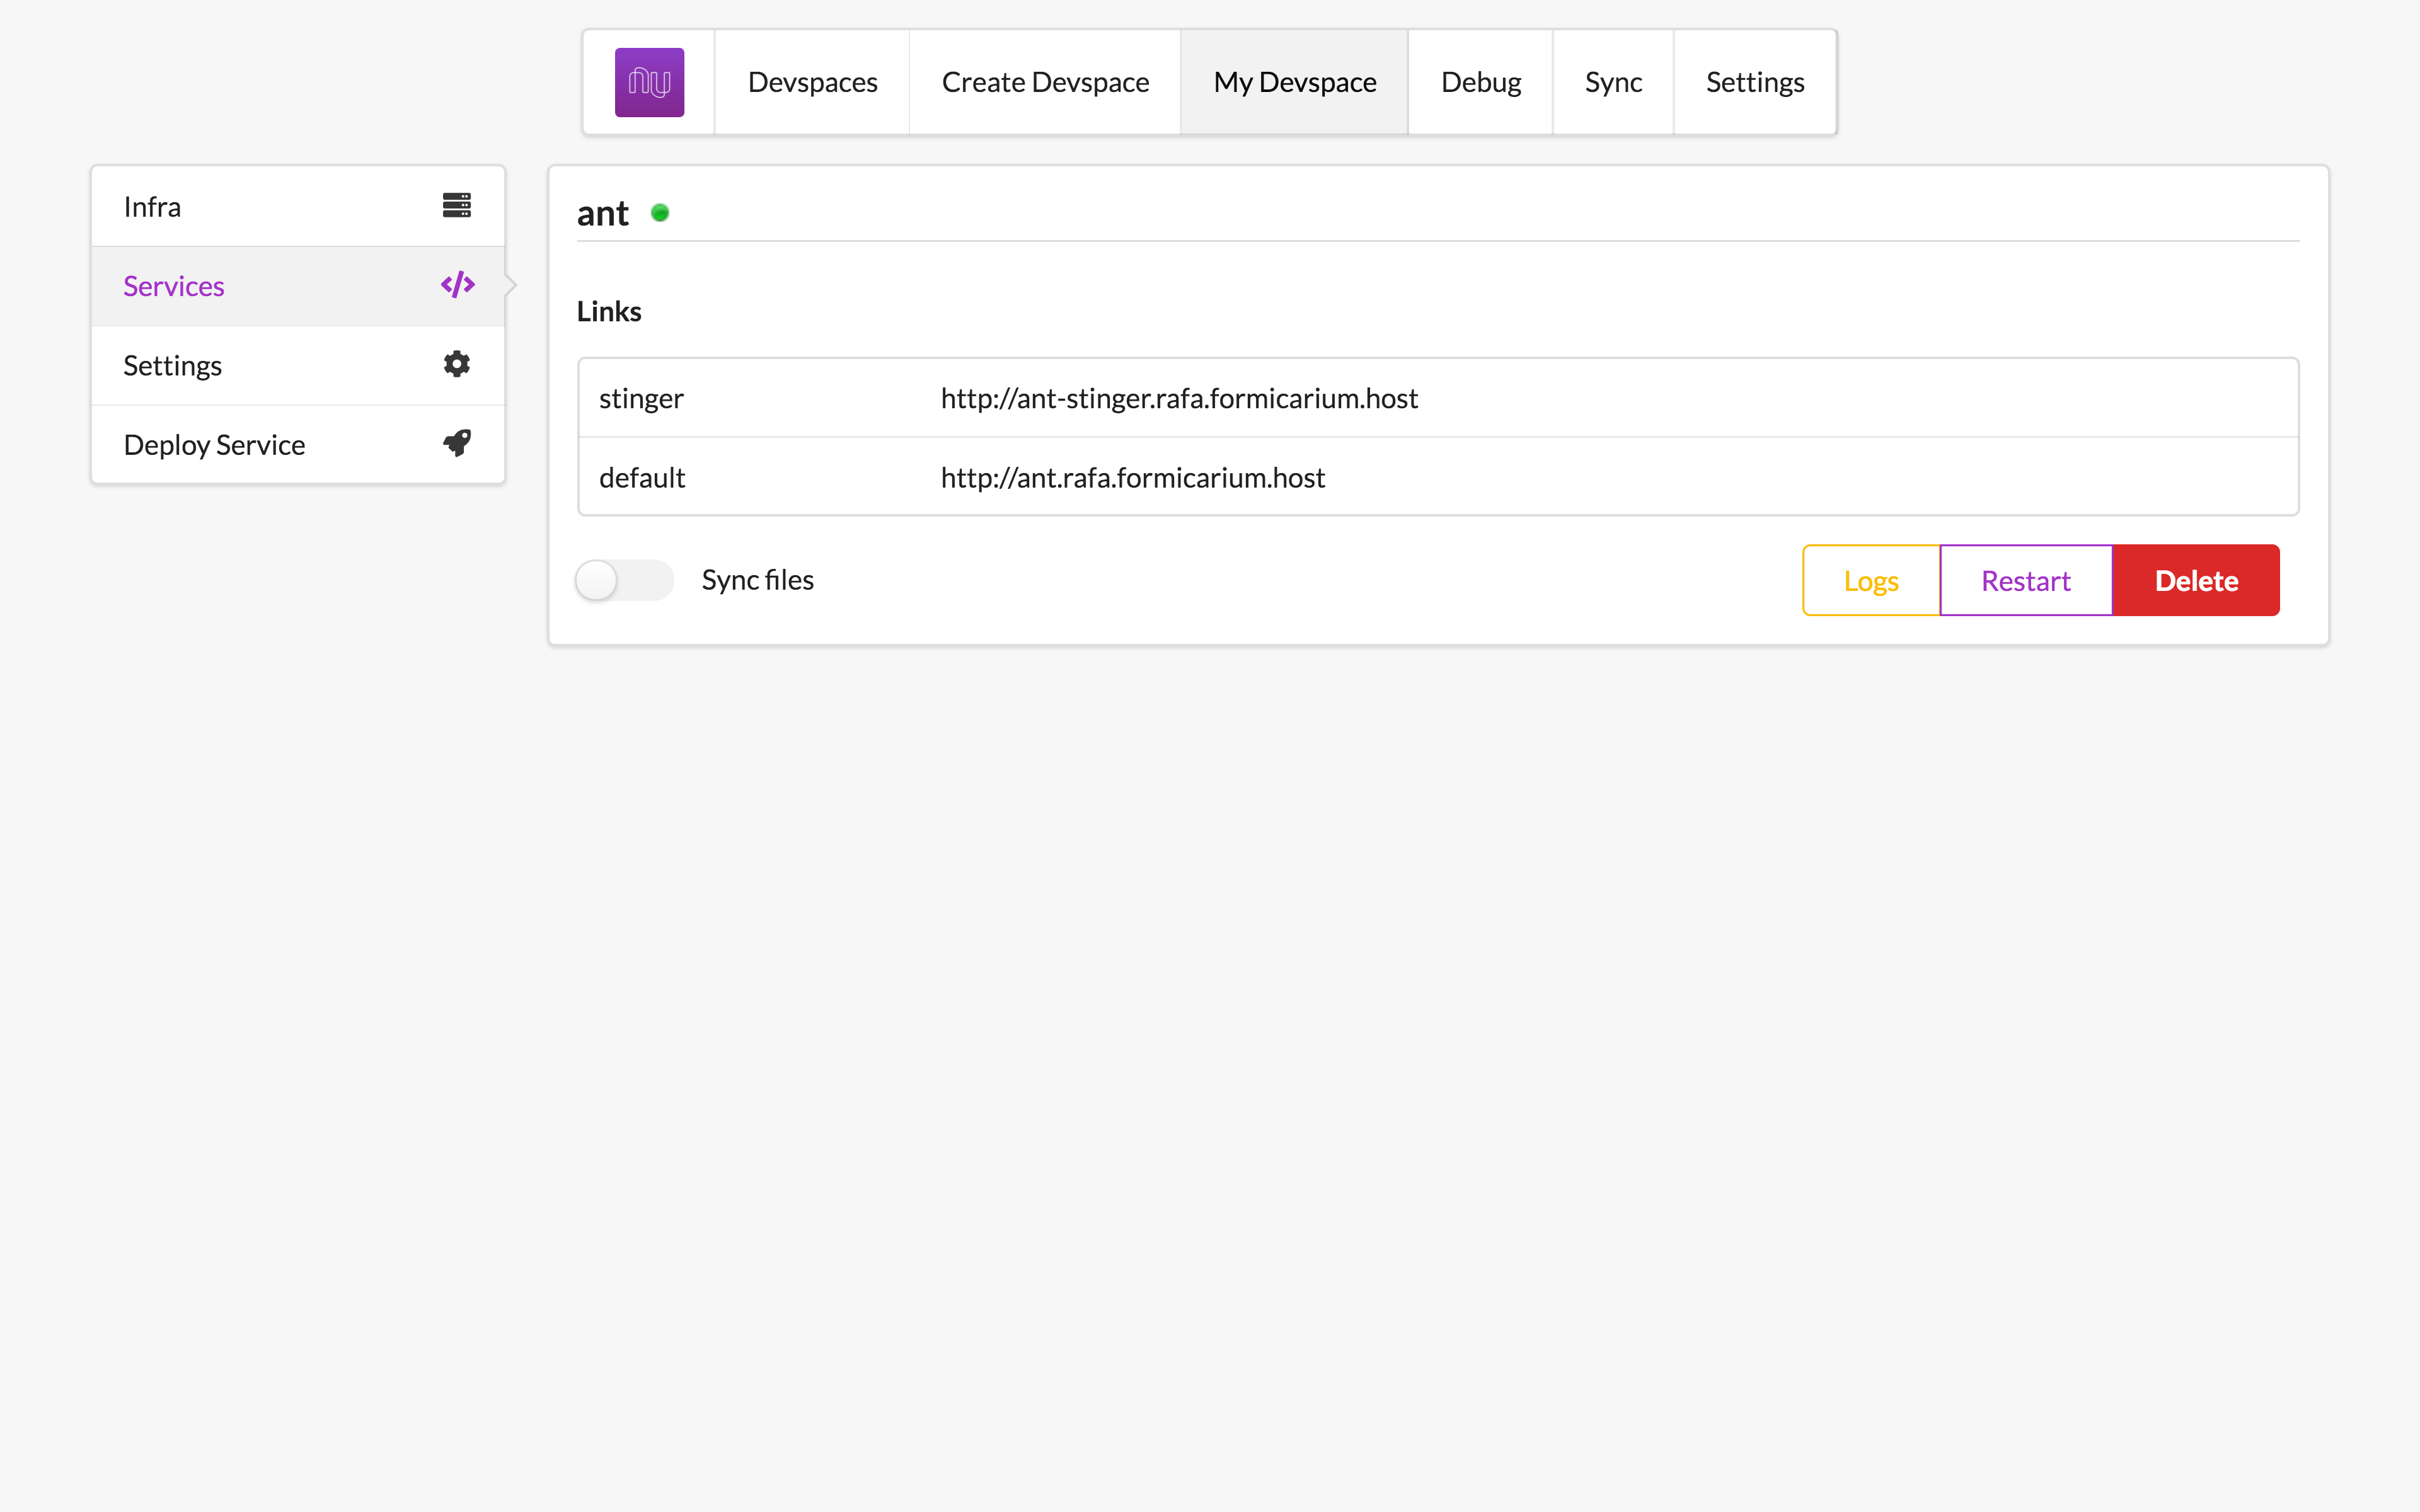
\includegraphics[width=\textwidth,keepaspectratio]{pictures/frontend/frontend-devspace-services.png}
	\end{center}
	\legend{Fonte: os autores - 2018-11-10}
\end{figure}

\begin{figure}[htb]
	\caption{\label{fig_frontend_logs}Tela Logs de um serviço}
	\begin{center}
	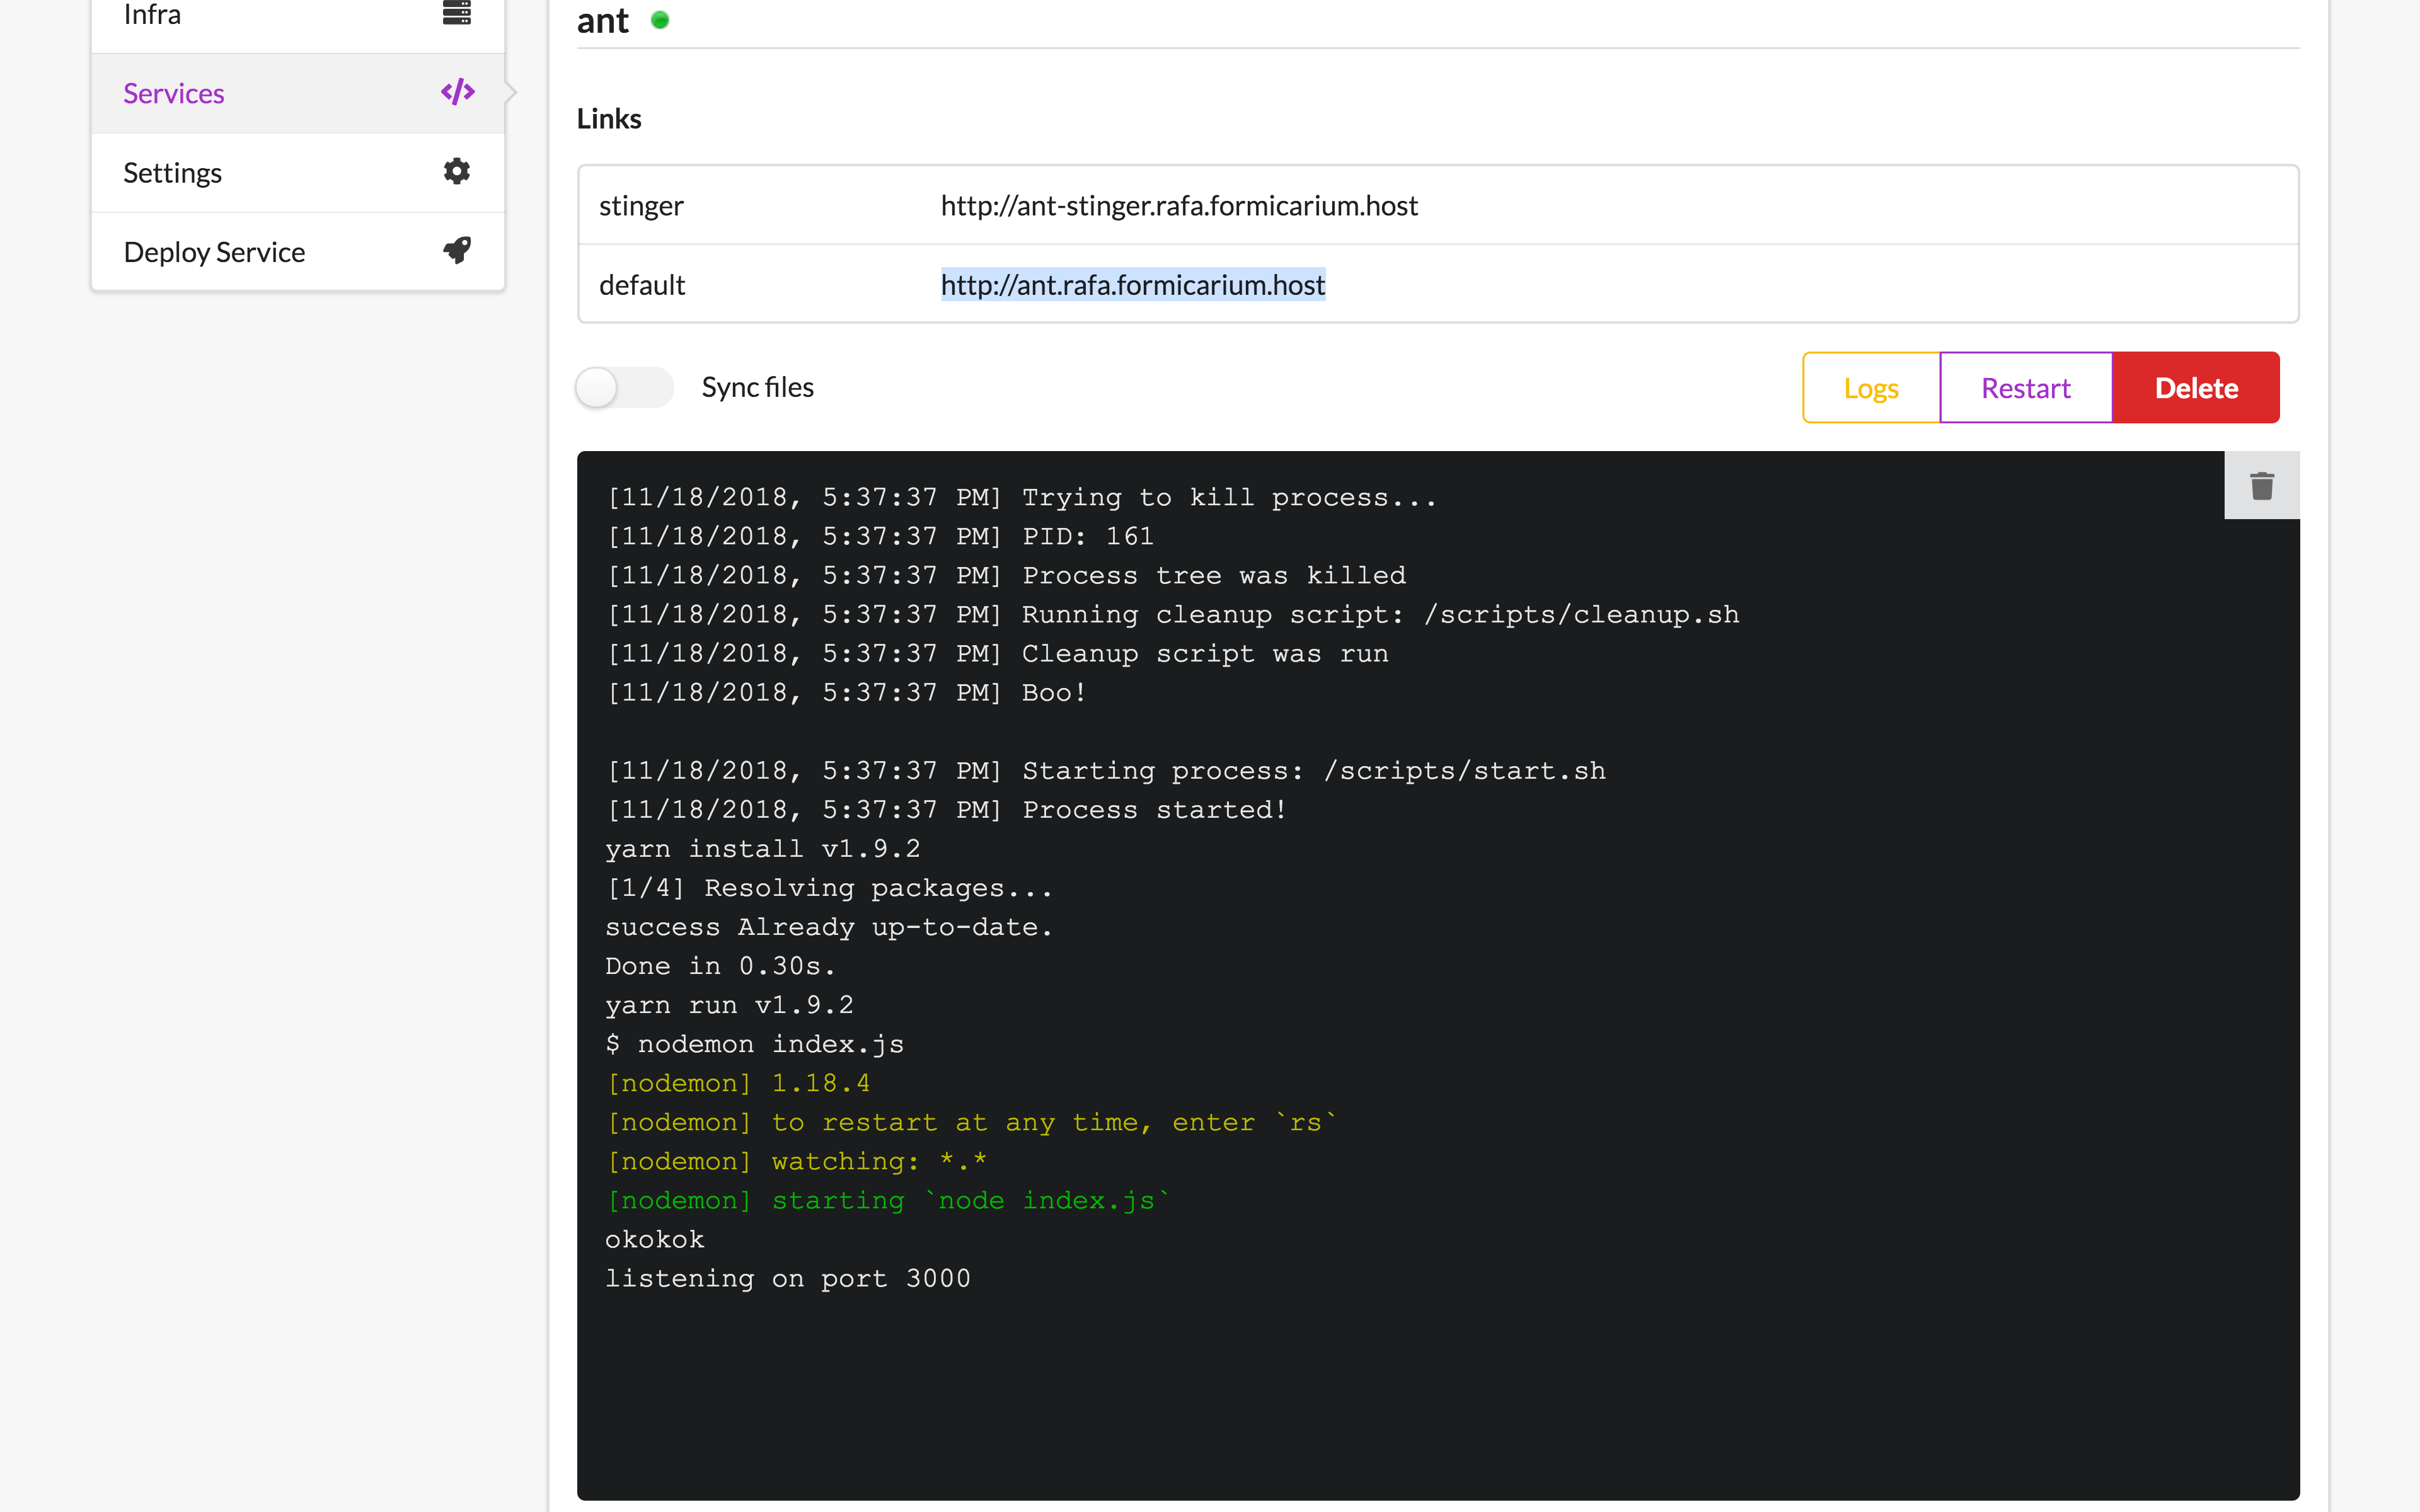
\includegraphics[width=\textwidth,keepaspectratio]{pictures/frontend/frontend-logs.png}
	\end{center}
	\legend{Fonte: Elaborado pelos autores}
\end{figure}

\subsubsection{Deploy}

Esta área conta com um formulário para implantação de um novo serviço. É possível inserir o nome, escolher se o serviço é do tipo \textit{Syncable} (o que fará com que a imagem Docker \textit{Chamber} seja usada). Caso esta opção esteja selecionada, o engenheiro deve apontar o diretório local em que está o código fonte do serviço para que este seja enviado para o contêiner remota e possa ser sincronizado em seguida.

\begin{figure}[htb]
	\caption{\label{fig_frontnd_deploy}Tela Deploy de serviços}
	\begin{center}
	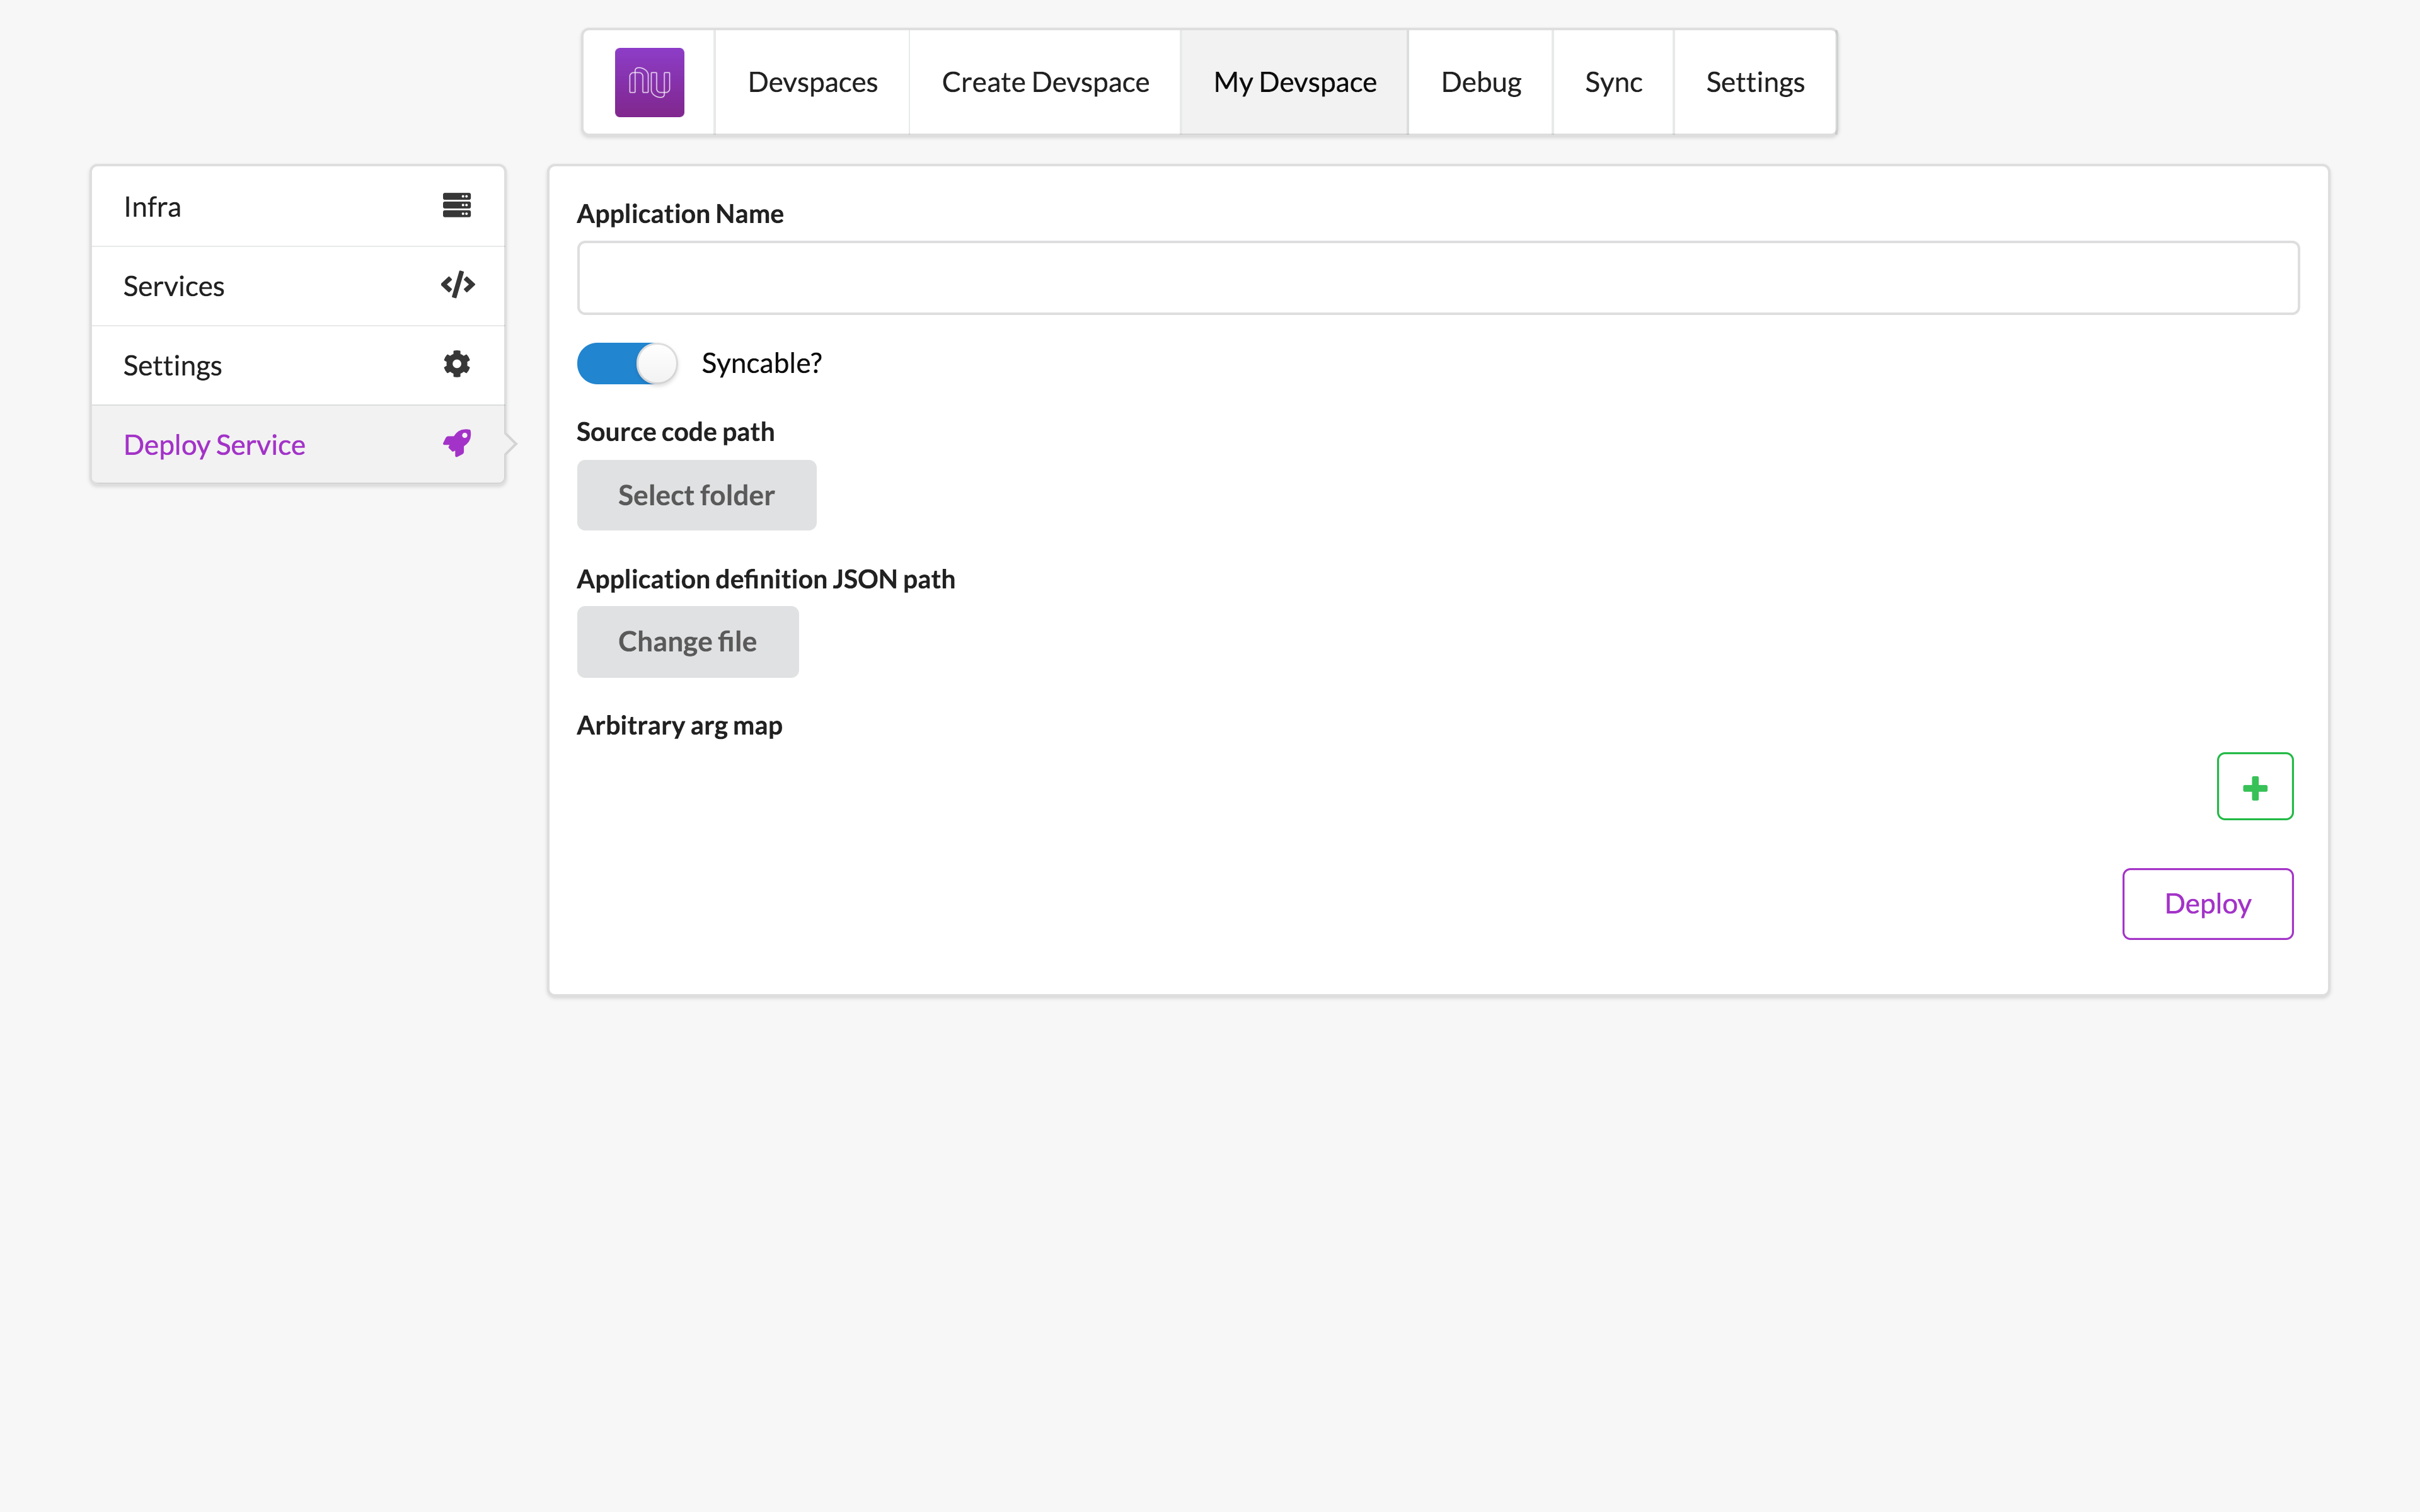
\includegraphics[width=\textwidth,keepaspectratio]{pictures/frontend/frontend-deploy.png}
	\end{center}
	\legend{Fonte: Elaborado pelos autores}
\end{figure}

\subsubsection{Distributed Debugger}

\subsubsection{Sync}

\subsubsection{Configurações}

\begin{figure}[htb]
		\caption{\label{fig_frontend_sync}Tela Sincronização de arquivos em um serviço}
		\begin{center}
		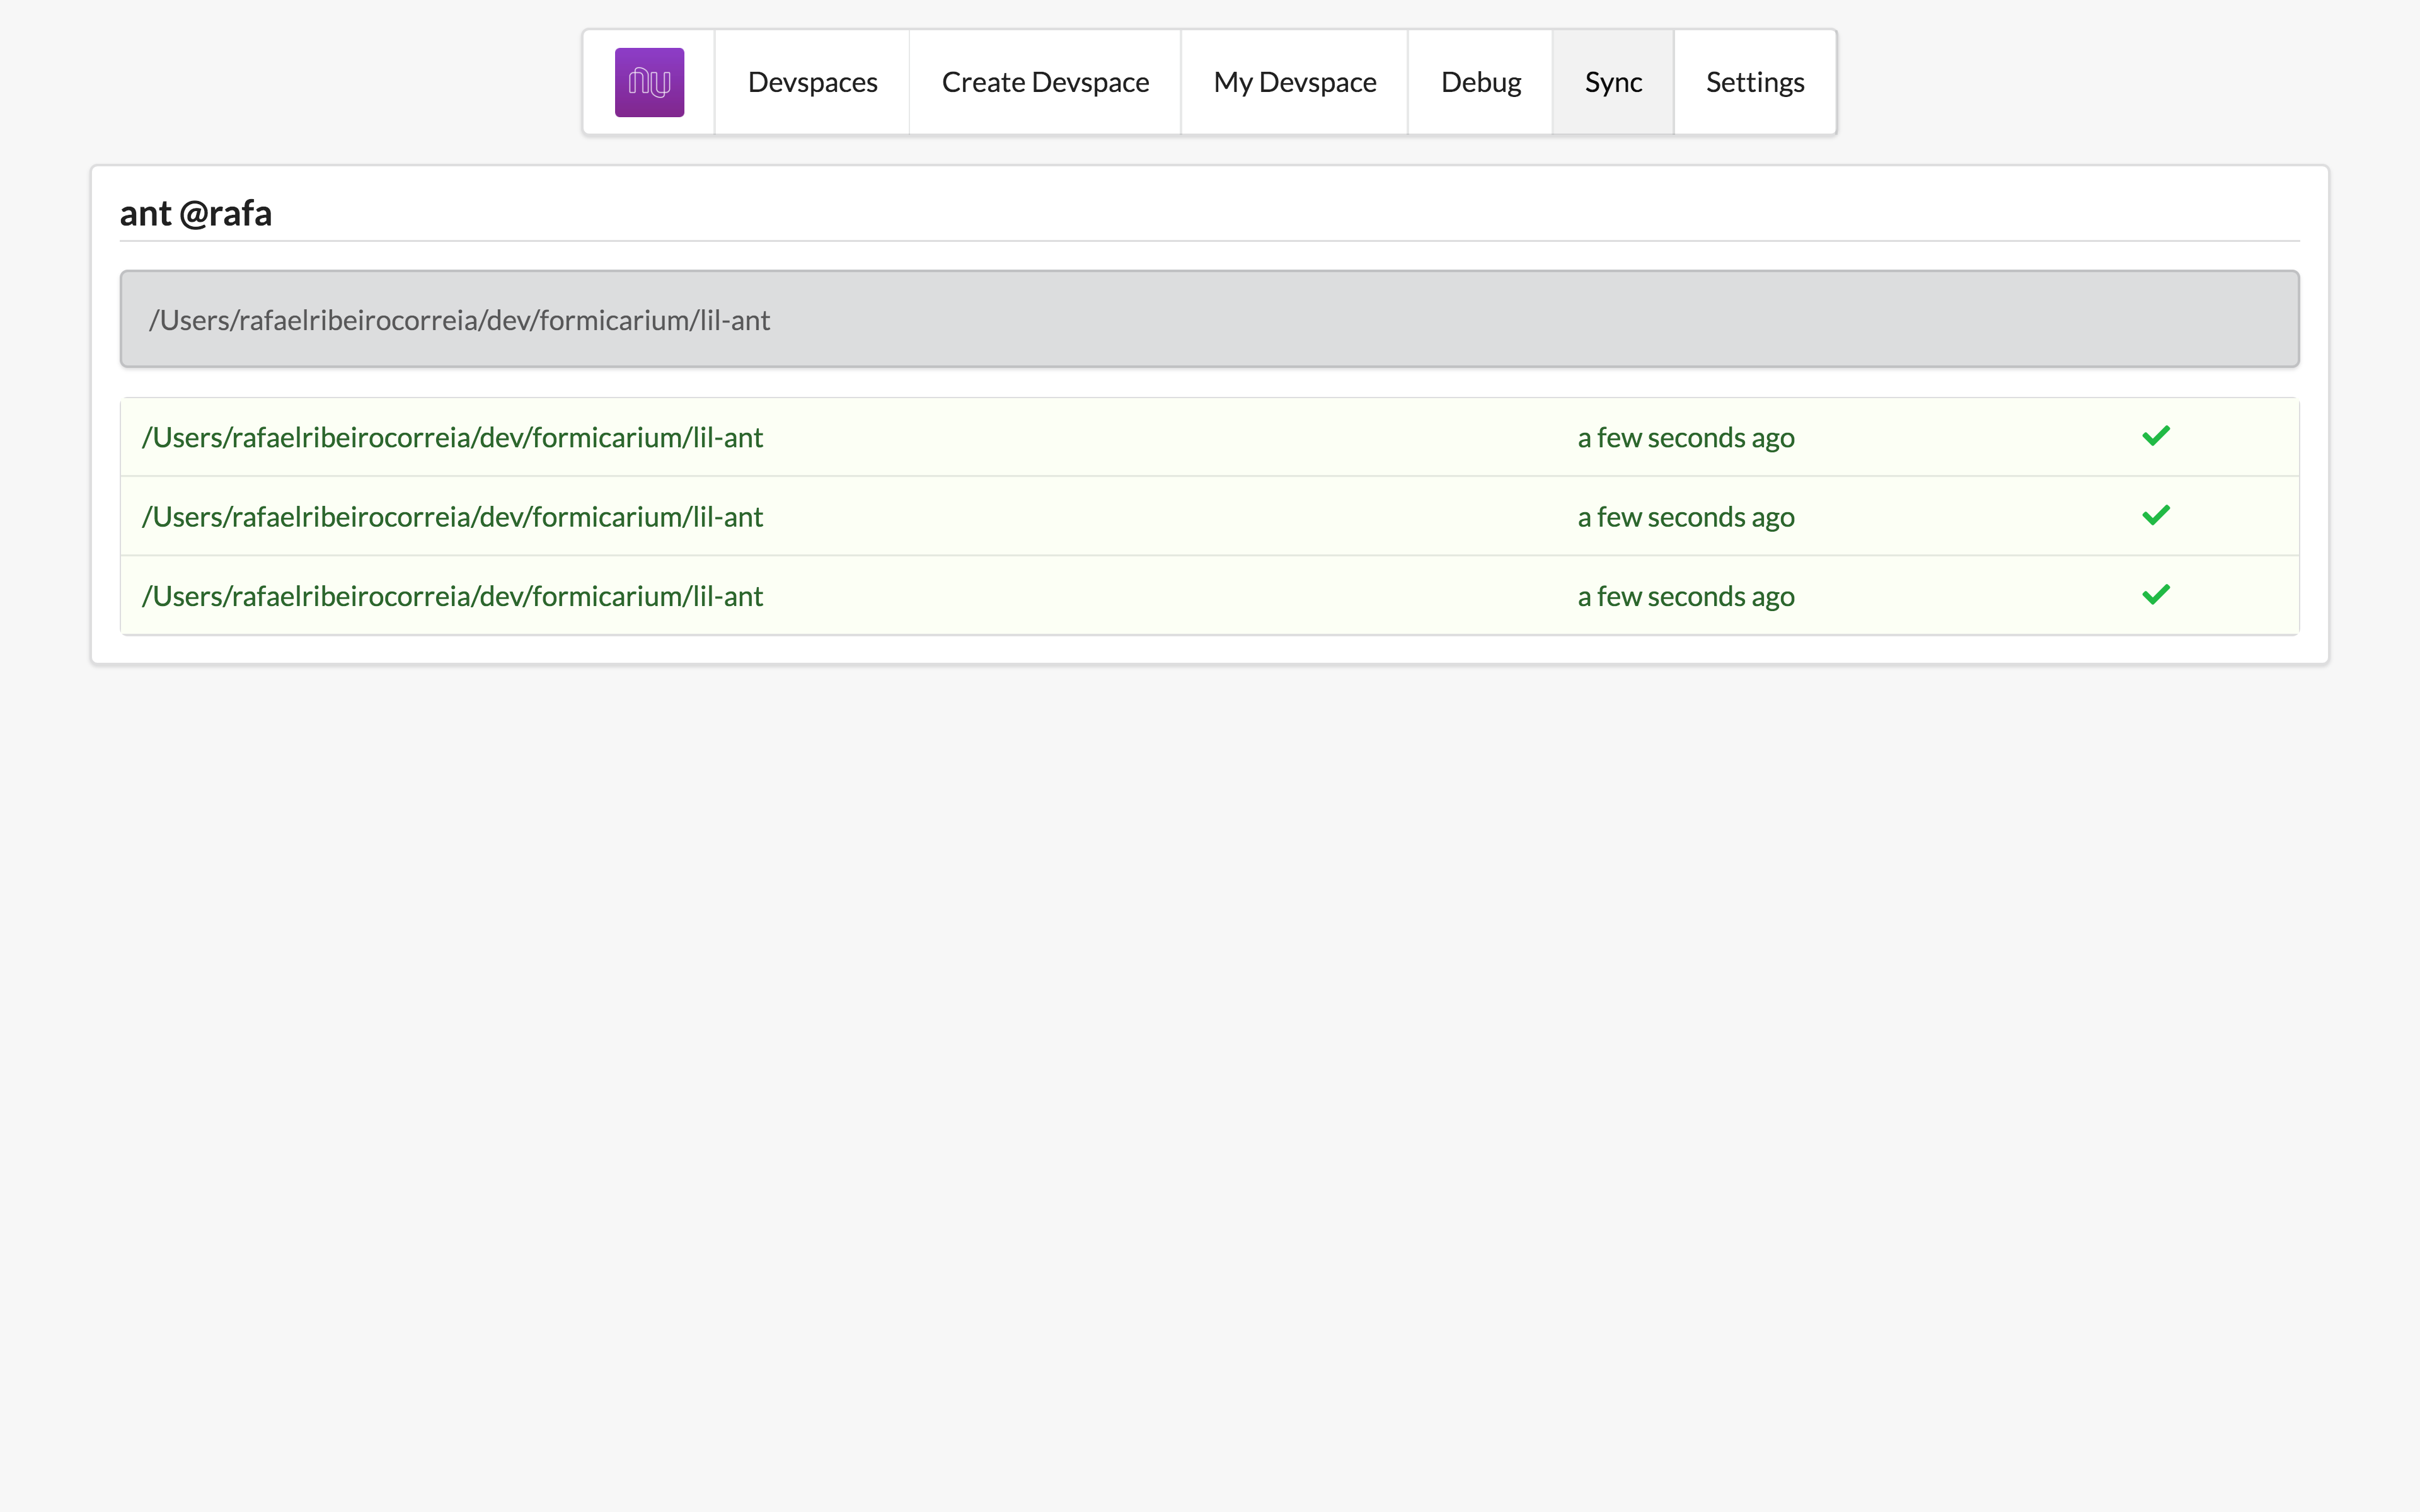
\includegraphics[width=\textwidth,keepaspectratio]{pictures/frontend/frontend-sync.png}
		\end{center}
		\legend{Fonte: Elaborado pelos autores}
	\end{figure}
	
\begin{figure}[htb]
		\caption{\label{fig_frontend_tracing_details}Tela Detalhes de uma requisição}
		\begin{center}
		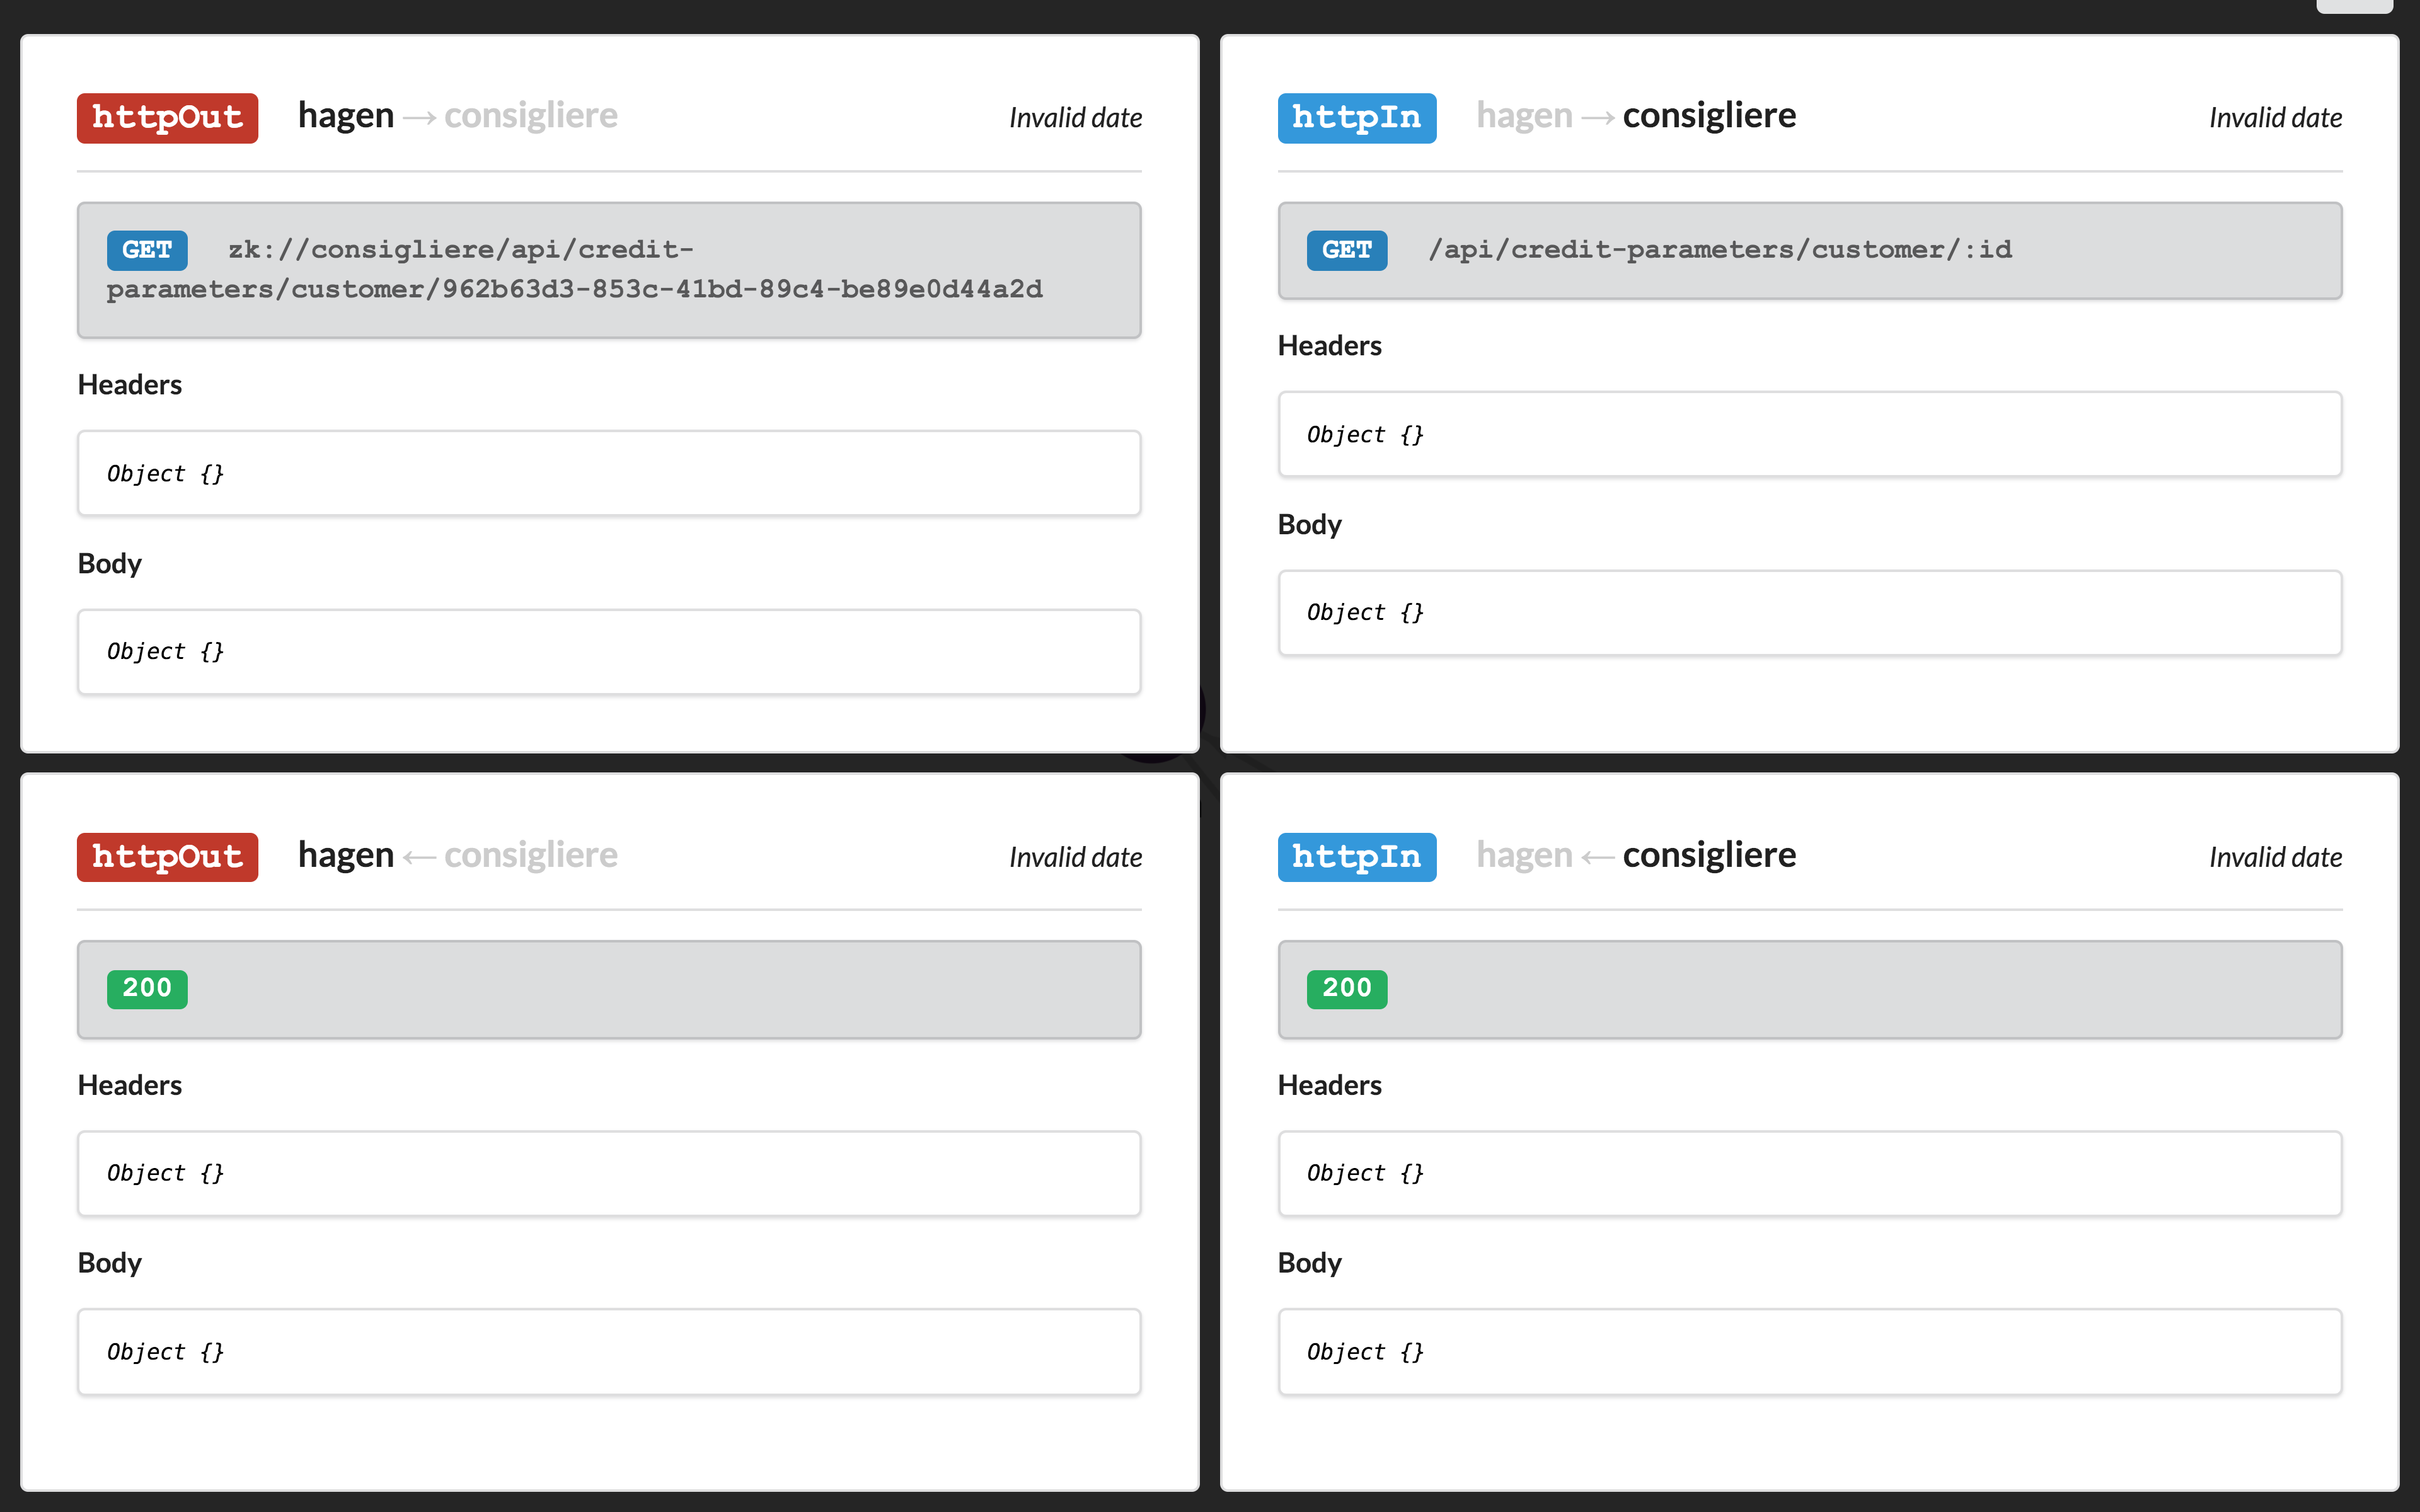
\includegraphics[width=\textwidth,keepaspectratio]{pictures/frontend/frontend-tracing-details.png}
		\end{center}
		\legend{Fonte: Elaborado pelos autores}
	\end{figure}
	
\begin{figure}[htb]
		\caption{\label{fig_frontend_tracing}Tela Grafo de interações em Tracing}
		\begin{center}
		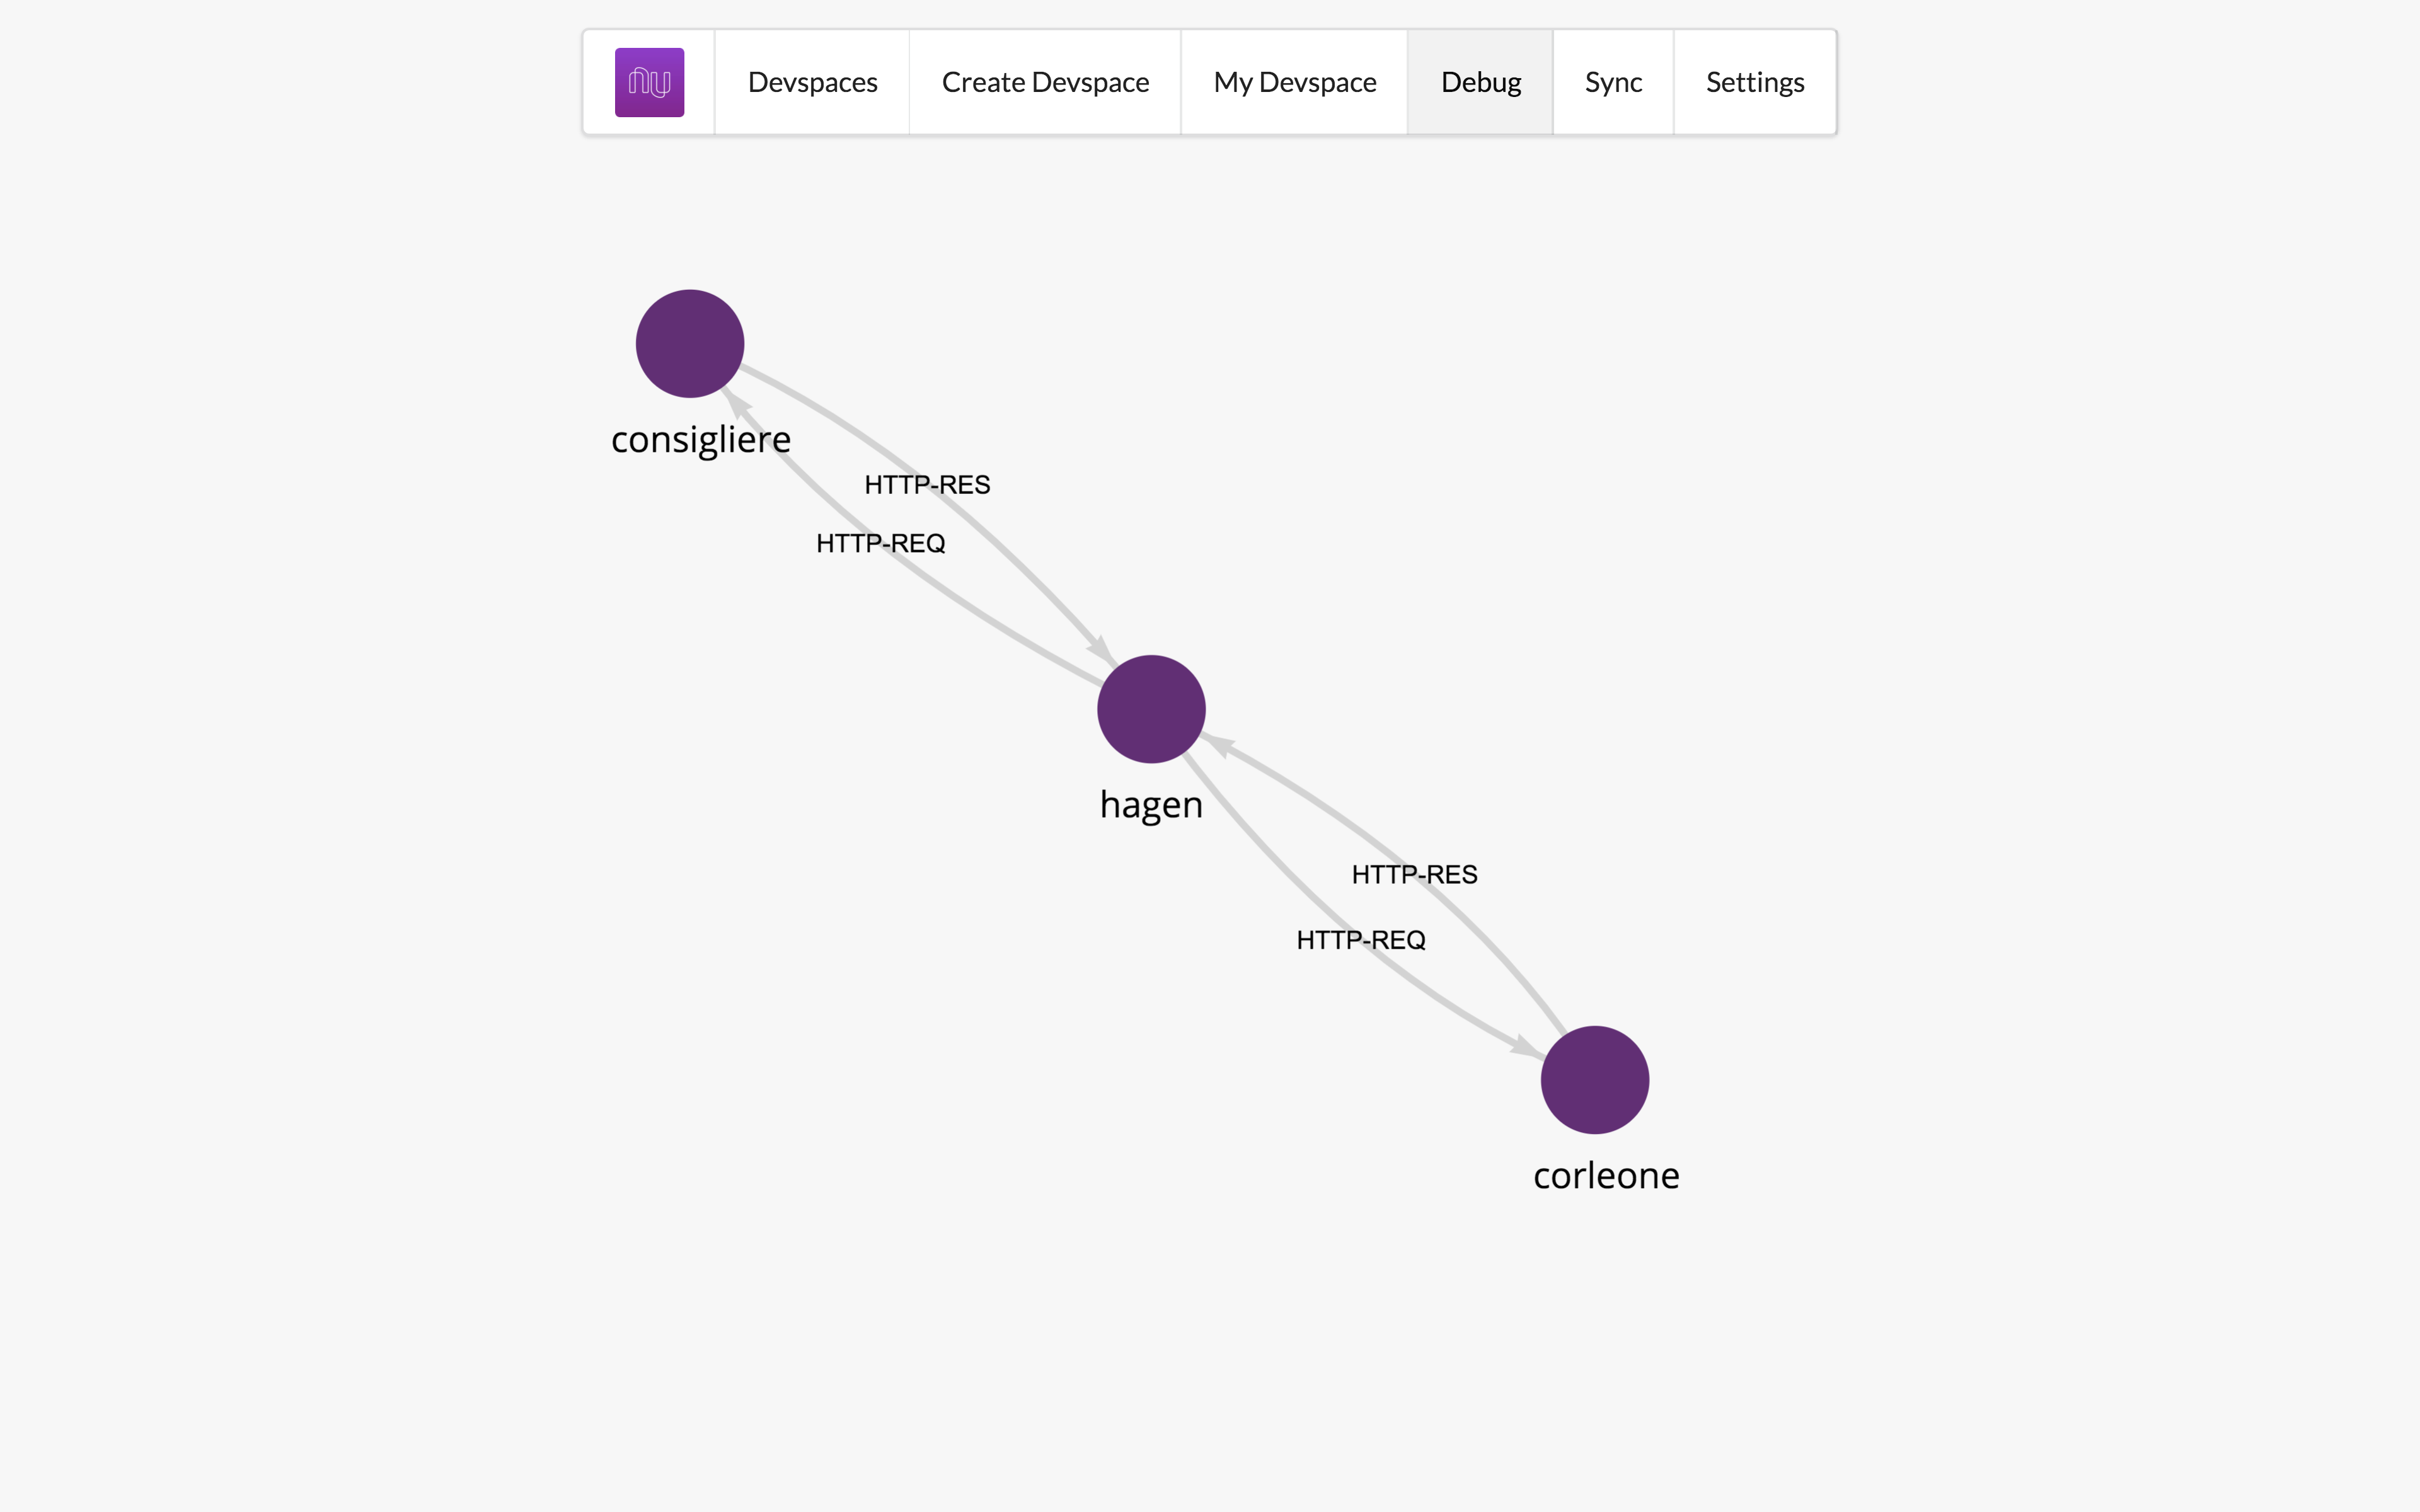
\includegraphics[width=\textwidth,keepaspectratio]{pictures/frontend/frontend-tracing.png}
		\end{center}
		\legend{Fonte: Elaborado pelos autores}
	\end{figure}

\begin{figure}[htb]
		\caption{\label{fig_frontend_create_devspace}Tela Criar novo Devspace}
		\begin{center}
		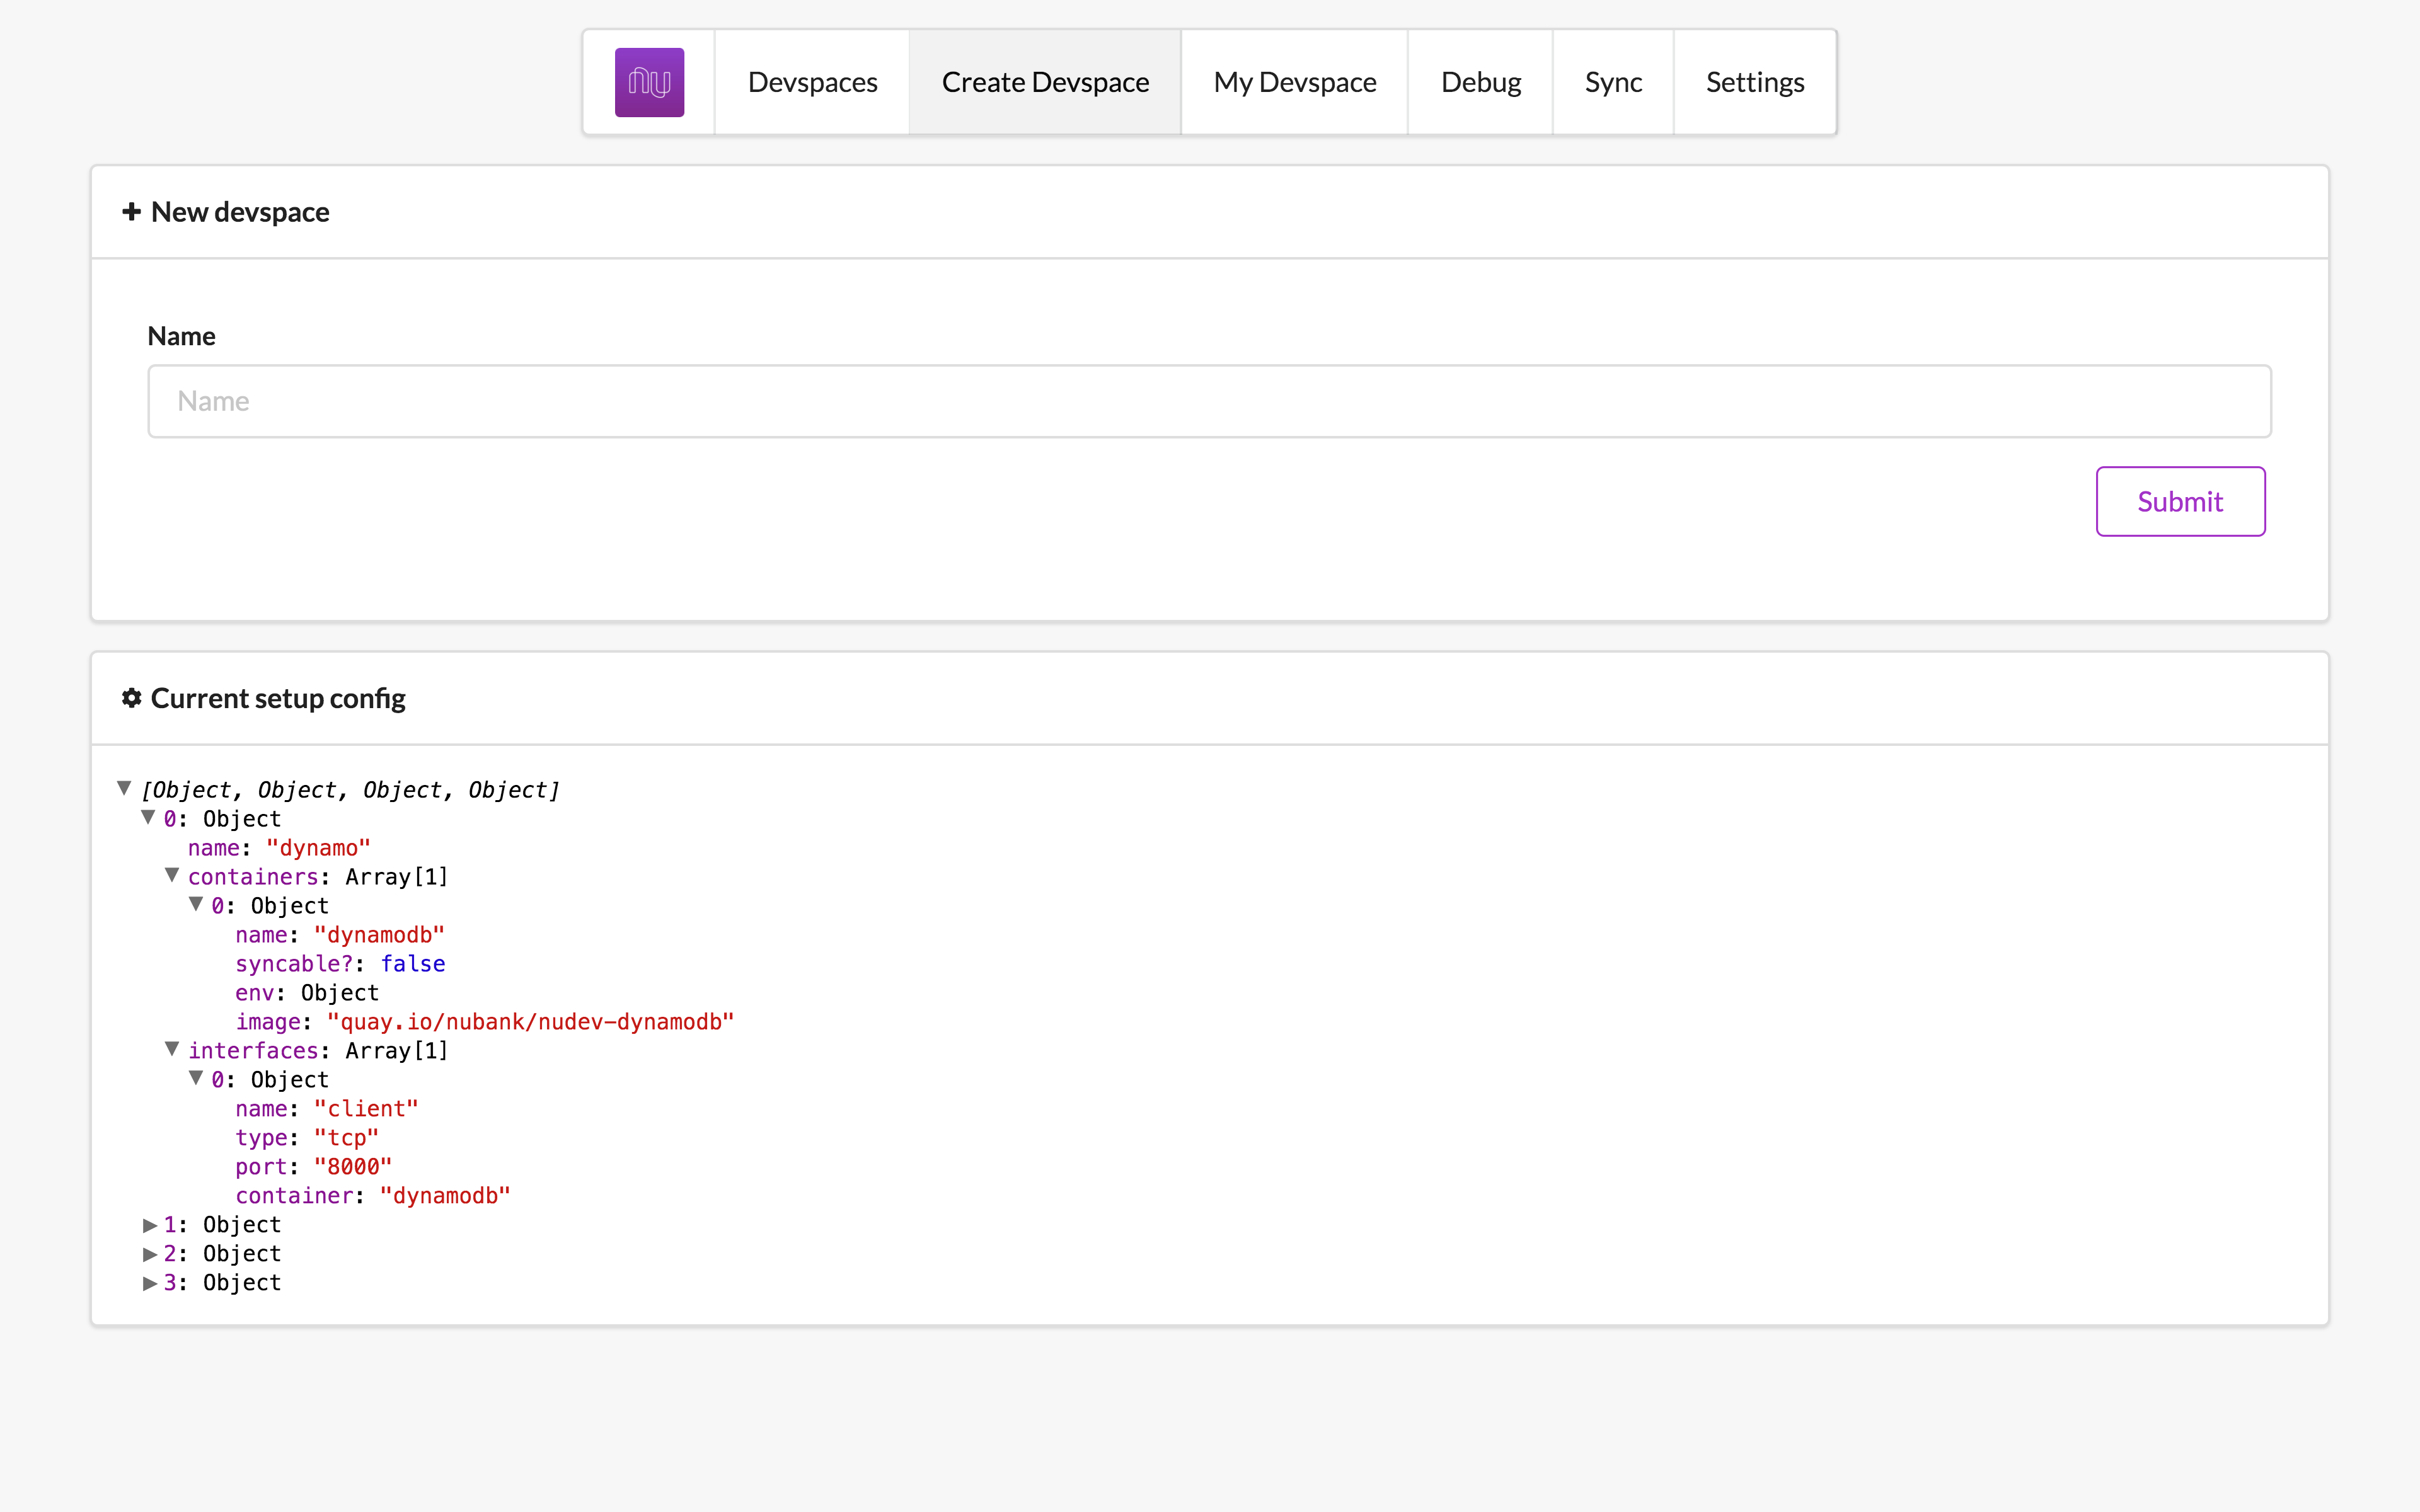
\includegraphics[width=\textwidth,keepaspectratio]{pictures/frontend/frontend-create-devspace.png}
		\end{center}
		\legend{Fonte: Elaborado pelos autores}
	\end{figure}
